\documentclass[thesis.tex]{subfiles}
\begin{document}

\chapter{Analyse der Kameras}
\label{chap:analysis}

\begin{figure}[h!]
\centering
\begin{subfigure}{.32\textwidth}
    \centering
    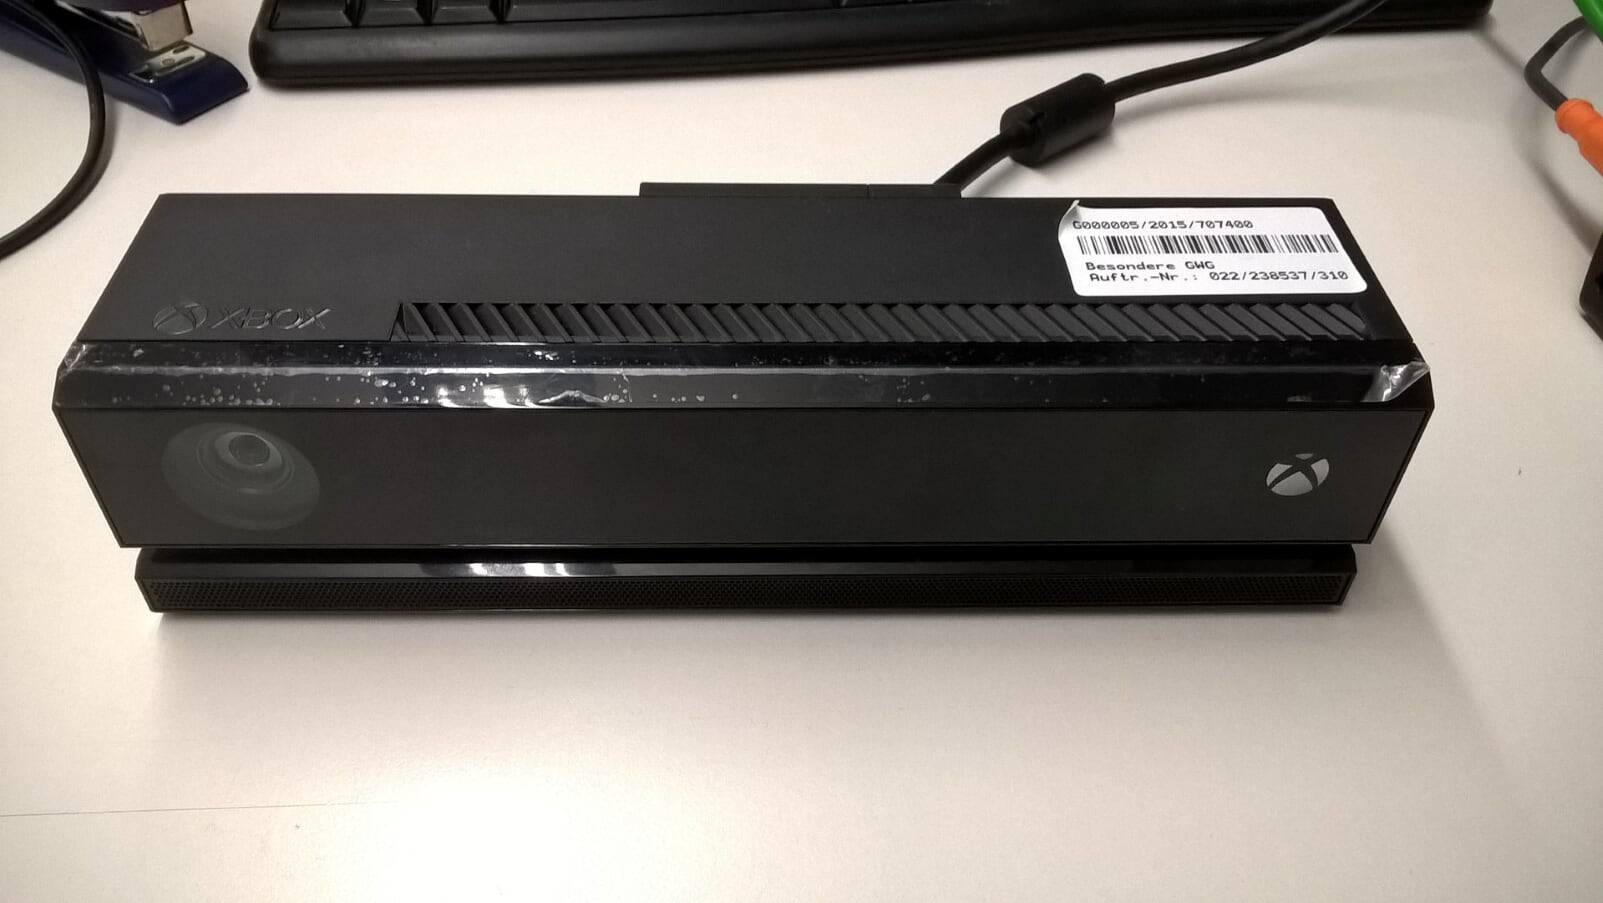
\includegraphics[width=.95\linewidth]{hardware/Hardware_Kinect}
    \caption{Microsoft Kinect v2}
    \label{fig:Hardware_Kinect}
\end{subfigure}%
\begin{subfigure}{.32\textwidth}
    \centering
    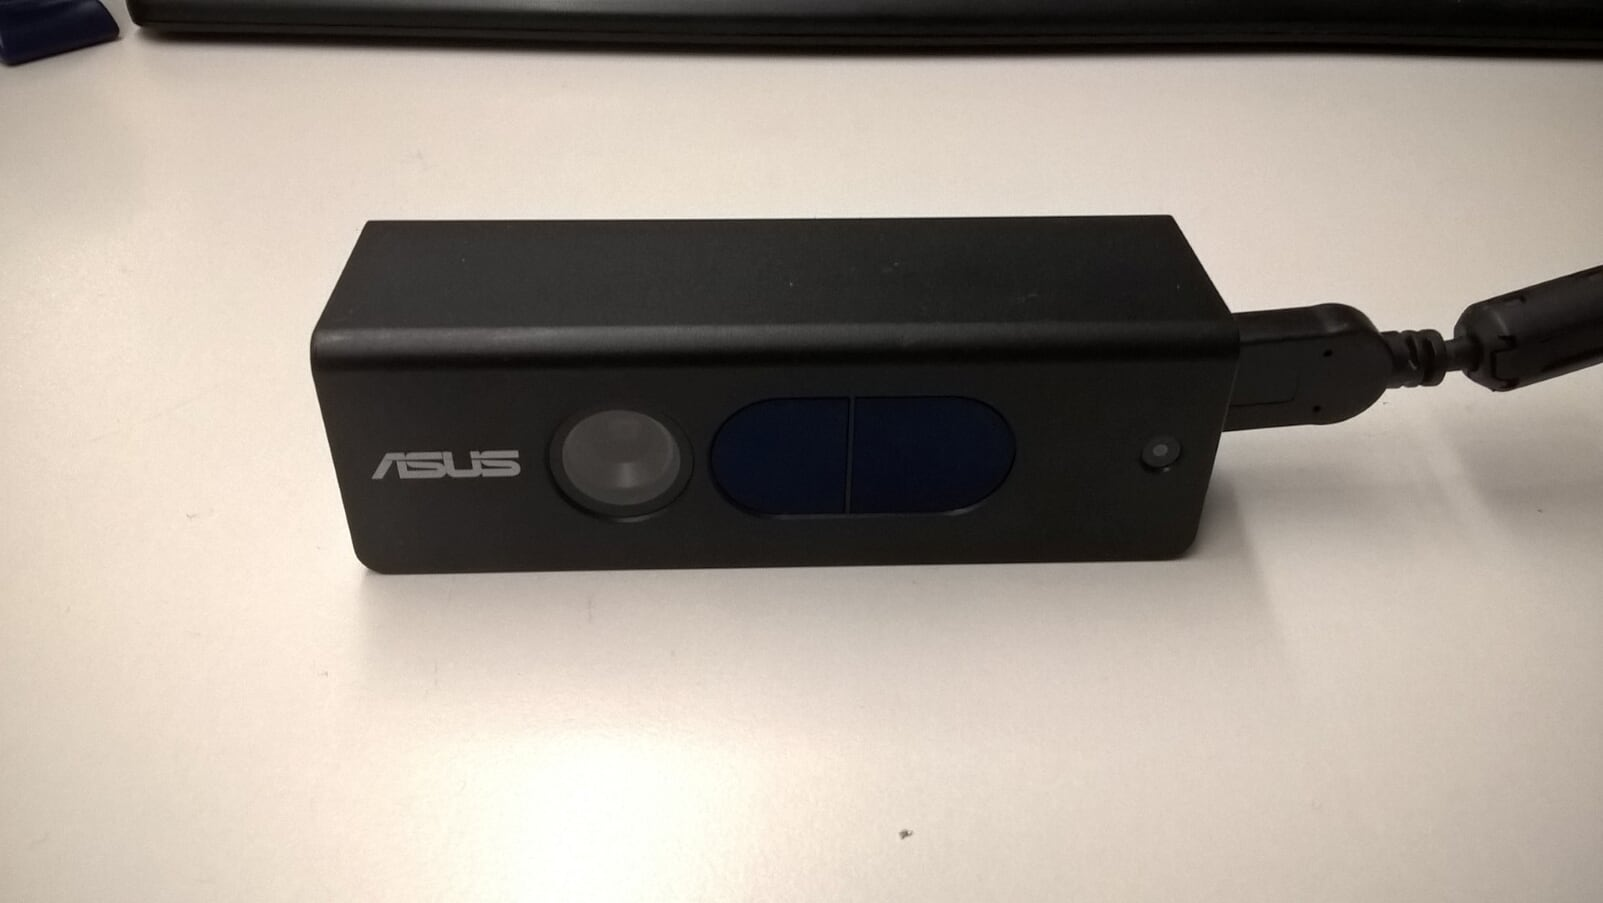
\includegraphics[width=.95\linewidth]{hardware/Hardware_Xtion2}
    \caption{ASUS Xtion 2}
    \label{fig:Hardware_Xtion2}
\end{subfigure}
\begin{subfigure}{.32\textwidth}
    \centering
    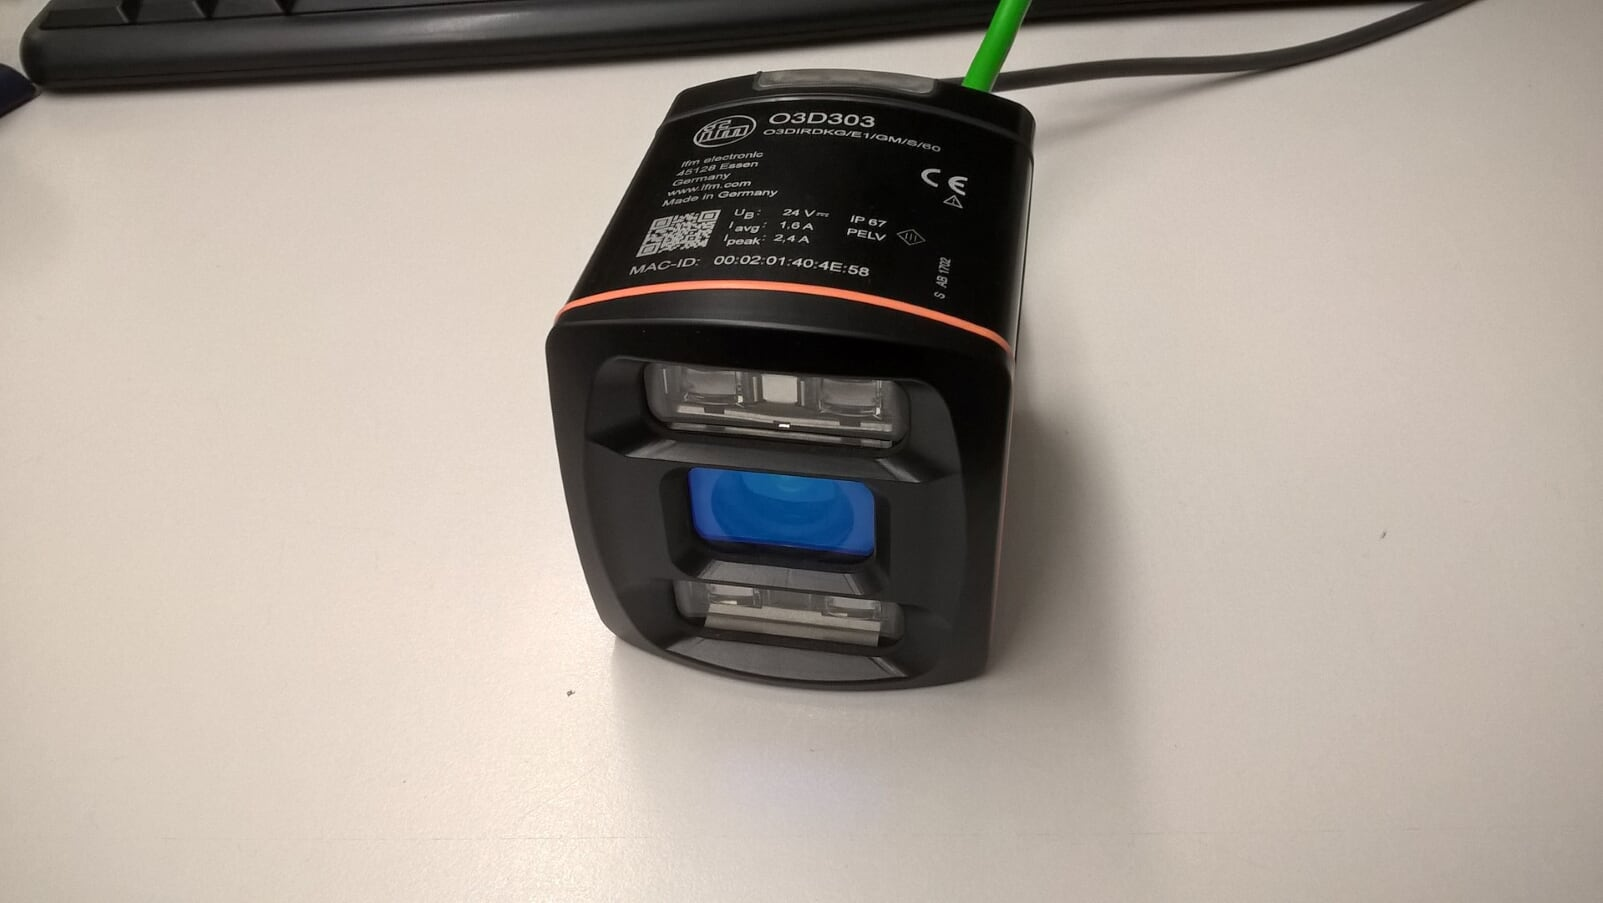
\includegraphics[width=.95\linewidth]{hardware/Hardware_IFM}
    \caption{IFM O3D303}
    \label{fig:Hardware_IFM}
\end{subfigure}
\end{figure}

Dieses Kapitel beschäftigt sich mit der Analyse der einzelnen Time-of-Flight Kamerasysteme, die im Rahmen der Arbeit genutzt werden. Dafür werden die Eigenschaften der IFM O3D303 (\autoref{fig:Hardware_IFM}), der Microsoft Kinect v2 (\autoref{fig:Hardware_Kinect}) und der Asus Xtion 2 (\autoref{fig:Hardware_Xtion2}) untersucht. In \autoref{tab:technicalspecifications} sind die vom Hersteller veröffentlichten technischen Daten der Kamerasysteme aufgelistet. Dabei ist anzumerken, dass es sich bei der Kinect v2 und der Xtion 2 um RGB-D Kamerasysteme handelt, in denen zusätzlich zum Time-of-Flight Sensor eine RGB Kamera verbaut wurde, während die O3D303 ausschließlich über einen Time-of-Flight Sensor verfügt. Die Kinect v2 liefert ein RGB Farbbild, ein Tiefenbild und ein Infrarotbild, während die Xtion 2 nur ein Farbbild und ein Tiefenbild und die O3D303 ein Tiefenbild und ein Infarotbild liefert. Die Kinect v2 und die Xtion 2 werden über USB 3.0 betrieben und die O3D303 wird über einen Netzwerkanschluss angesprochen, über den die Daten gesendet werden. Da, wie in \autoref{chap:cw_tof} erläutert, die Mehrdeutigkeitsdistanz in direkter Relation zur genutzten Frequenz steht, wurde anhand der gemessenen Maximaldistanz des Tiefenbildes für die O3D303 eine Frequenz von 30 Mhz und für die Xtion 2 eine Frequenz von 20 Mhz für die genutzte Wellenfunktion festgestellt.
%
\begin{table}[h!]
\centering
\caption{Technische Spezifikationen der Time-of-Flight Kamerasysteme}
\begin{tabular}{|c|c|c|c|}
    \hline
    Gerät & Kinect v2 & Xtion 2 & O3D303 \\
    \hline
    Auflösung Farbbild      & 1920 x 1080 & 2592 x 1944 & - \\
    Auflösung Tiefenbild    & 512 x 424 & 640 x 480 & 352 x 264 \\
    Framerate Tiefenbild    & 30 fps & 30 fps & 4 - 25 fps  \\
    Zugriff auf IR Aufnahmen & Ja & Nein & Ja \\
    Field of View Tiefenbild & \ang{70} x \ang{60} & \ang{74} x \ang{52} & \ang{60} x \ang{45}\\
    Reichweite              & 0,5 - 4,5 m & 0,8 - 3,5 m & 0,3 - 30 m \\
    \hline
\end{tabular}
\label{tab:technicalspecifications}
\end{table}
%
Keine der Kameras verfügt über einen einstellbaren Fokus oder eine einstellbare Blendenöffnung. Die O3D303 erlaubt allerdings eine feinere Konfiguration der Belichtungszeiten und weitere Konfigurationsmöglichkeiten, wie das Nutzen von wahlweise bis zu drei verschiedenen Frequenzen und drei Belichtungsmodi, in denen mehrere Bilder mit unterschiedlichen Belichtungszeiten erstellt werden, um eine hohe Belichtung und damit verbunden geringes Rauschen zu ermöglichen, ohne die Sensoren dabei überzubelichten. In der vorliegenden Arbeit wird für die Evaluation der O3D303 nur eine Frequenz von 30 Mhz und der einfachste Belichtungsmodus verwendet, in dem nur eine Aufnahme mit variabler Belichtungszeit gemacht wird.

In den folgenden Unterkapiteln werden die einzelnen Kamerasysteme auf ihre Eigenschaften und auf die Beeinflussung des Tiefenbildes durch die Lichtausbreitung untersucht. Es sei angemerkt, dass zur besseren Unterscheidung die Graphen einem festen Schema folgen: Die Datensätze der Kinect v2 werden durch blaue Quadrate dargestellt, während für die Xtion 2 rote Kreise und für O3D303 schwarze Dreiecke verwendet werden.
%
\subsection{Radiale Verzeichnung}\label{sec:radial_distortion}
%
\begin{figure}[h!]
\centering
\begin{subfigure}{.32\textwidth}
    \centering
    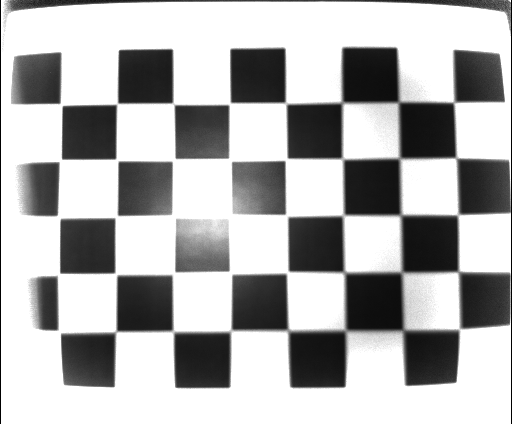
\includegraphics[width=.95\linewidth]{evaluation/Kinect_v2/IR_0_512_424}
    \caption{Microsoft Kinect v2}
    \label{fig:Kinect_v2_Checkerboard}
\end{subfigure}%
\begin{subfigure}{.32\textwidth}
    \centering
    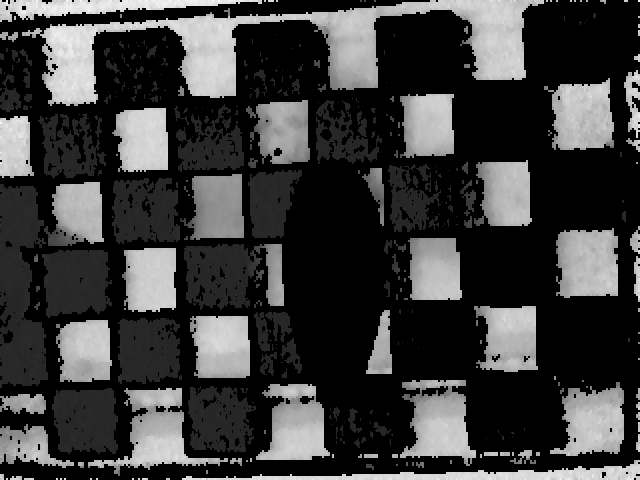
\includegraphics[width=.95\linewidth]{evaluation/Xtion_2/Depth_14_640_480}
    \caption{ASUS Xtion 2}
    \label{fig:Xtion_2_Checkerboard}
\end{subfigure}
\begin{subfigure}{.32\textwidth}
    \centering
    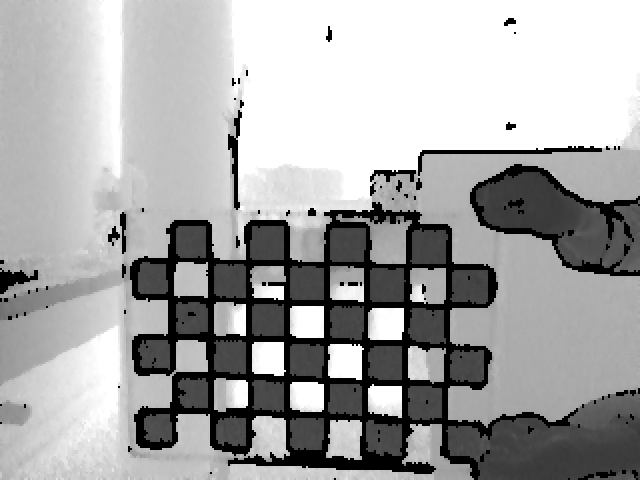
\includegraphics[width=.95\linewidth]{evaluation/O3D303/checkerboard}
    \caption{IFM O3D303}
    \label{fig:IFM_O3D303_Checkerboard}
\end{subfigure}
\caption{Radiale Verzeichnung der Infrarotkameras, die mittels Schachbrettmustern veranschaulicht werden.}
\end{figure}

Die monokulare Kamera Kalibrierung kann als bereits \glq gelöstes Problem\grq{} betrachtet werden und unter Verwendung der durch OpenCV angebotenen Algorithmen durchgeführt werden \cite{bib:Hertzberg2014}. Diese Arbeit verwendet Schachbrettmuster zur Kalibrierung der RGB und Infrarotkameras, um die \emph{radiale Verzeichnung} oder \emph{radial distortion} zu ermitteln. Als radiale Verzeichnung wird der geometrische Abbildungsfehler optischer Systeme bezeichnet, der duch die Linsenkrümmung verursacht wird. Die Abweichung des Kamerabildes vom linearen Kameramodell kann mit Hilfe eines bekannten Schachbrettmusters ermittelt werden. Durch die Kalibrierung werden außerdem die Brennweite und das optische Zentrum der Kamera bestimmt, die zur Schätzung der Position und Orientierung von ArUco Markern benötigt werden, die in den nächsten Unterkapiteln Verwendung thematisiert werden.

\begin{figure}[h!]
\centering
\begin{subfigure}{.32\textwidth}
    \centering
    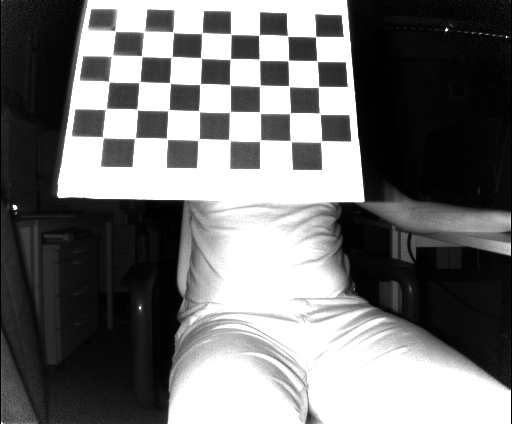
\includegraphics[width=.95\linewidth]{evaluation/Kinect_v2/IR_2_512_424}
\end{subfigure}%
\begin{subfigure}{.32\textwidth}
    \centering
    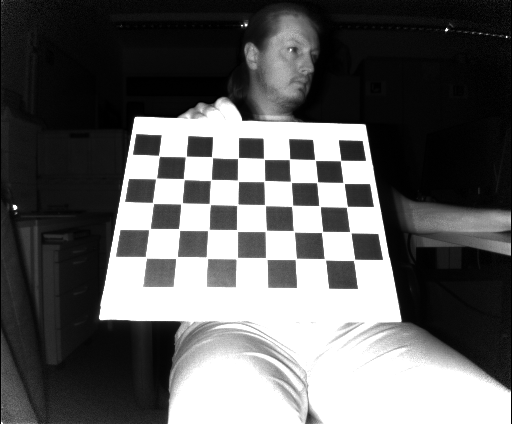
\includegraphics[width=.95\linewidth]{evaluation/Kinect_v2/IR_5_512_424}
\end{subfigure}
\begin{subfigure}{.32\textwidth}
    \centering
    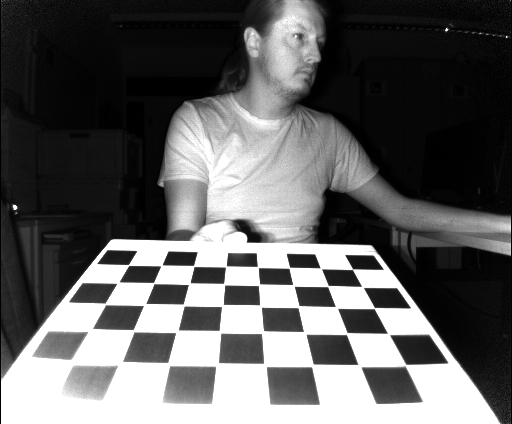
\includegraphics[width=.95\linewidth]{evaluation/Kinect_v2/IR_10_512_424}
\end{subfigure}
\caption{Auszug der Schachbrettaufnahmen, die zur Kalibrierung der Kinect v2 verwendet wurden.}
\label{fig:checkerboard_kinect_ir}
\end{figure}

Bei dem Schachbrettmuster handelt es sich um ein 8 mal 5 Schachbrett mit exakt quadratischen Feldern mit einer Kantenlänge von jeweils 32mm. Zur Kalibrierung wurden für jede Infrarotkamera zwischen 60 bis 80 Aufnahmen in unterschiedlichen Orientierungen und Positionierungen des Schachbretts erstellt (siehe \autoref{fig:checkerboard_kinect_ir}). Für die Xtion 2 musste eine transparente Folie mit einem Schachbrettmuster bedruckt werden, welche an einer Plexiglasscheibe angebracht wurde, da die Xtion 2 keinen Zugriff auf das Infarotbild liefert (siehe \autoref{fig:Xtion_2_Checkerboard}). Daher sind in der Abbildung Blendflecke zu sehen, die durch die Spiegelungen an der Plexiglasscheibe entstanden sind. Statt des Infarotbildes wurde deshalb das Tiefenbild zum Kalibrieren der Tiefenbildkamera verwendet. Das Ergebnis der Kalibrierung wird in Form einer Kameramatrix und Verzeichnungskoeffizienten ausgegeben, mit deren Hilfe sich die Verzeichnung beheben und das Kamerabild in ein lineares Kameramodell überführen lässt.

Die Kameramatrix wird folgendermaßen definiert:
\begin{equation}
C_{matrix} = \begin{bmatrix}
    f_x & 0 & c_x\\
    0 & f_y & c_y\\
    0 & 0   & 1
\end{bmatrix}
\end{equation}
wobei $f_x$ und $f_y$ die Brennweite und $c_x$ und $c_y$ das optische Zentrum in Pixelkorrdinaten darstellen. Die Verzeichnungskoeffizienten werden als 4-, 5-, oder 8-Tupel übergeben:
\begin{equation}
D_{coefficients} = (k_1, k_2, p_1, p_2[, k_3[, k_4, k_5, k_6]]),
\end{equation}
wobei in dieser Untersuchung ausschließlich 5-Tupel verwendet werden. Mit Hilfe der Kameramatrix und den Verzeichnungskoeffizienten kann nun für jede Pixelkoordinate $(u, v)$ eine entzerrte Pixelkoordinate $(u', v')$ bestimmt werden. Hier wird dafür auf die Implementierung von OpenCV zurückgegriffen:
%
\begin{equation}
\begin{aligned}
x^{'} &\leftarrow (u - c_x)/f_x \\
y^{'} &\leftarrow (v - c_y)/f_y \\
(u',v') &= undistort(x^{'},y^{'}, D_{coefficients}).
\end{aligned}
\end{equation}

\begin{figure}[h!]
\centering
\begin{subfigure}{.32\textwidth}
    \centering
    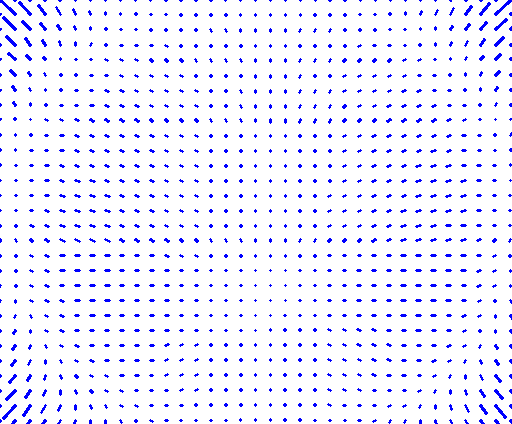
\includegraphics[width=.95\linewidth]{evaluation/Kinect_v2/Kinect_v2_Calibration}
    \caption{Microsoft Kinect v2}
    \label{fig:Kinect_v2_Calibration}
\end{subfigure}%
\begin{subfigure}{.32\textwidth}
    \centering
    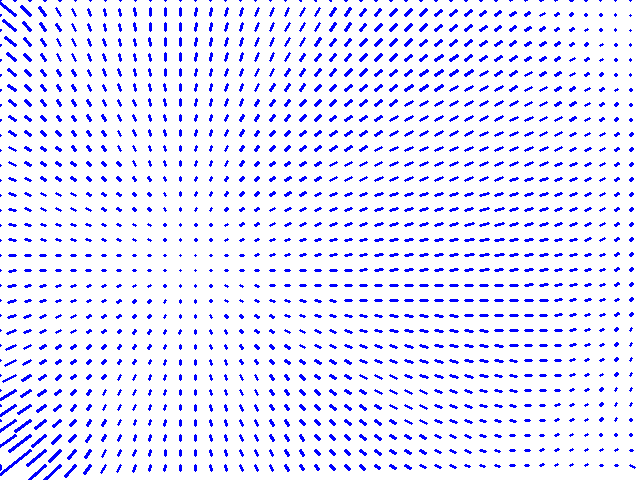
\includegraphics[width=.95\linewidth]{evaluation/Xtion_2/Xtion_2_Calibration}
    \caption{ASUS Xtion 2}
    \label{fig:Xtion_2_Calibration}
\end{subfigure}
\begin{subfigure}{.32\textwidth}
    \centering
    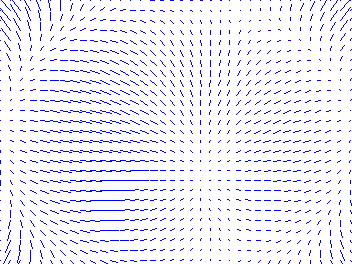
\includegraphics[width=.95\linewidth]{evaluation/O3D303/IFM_O3D303_Calibration}
    \caption{IFM O3D303}
    \label{fig:IFM_O3D303_Calibration}
\end{subfigure}
\caption{Ergebnis der Kalibrierung und Darstellung der radialen Verzeichnung der Infrarotkameras.}
\label{fig:camera_correction}
\end{figure}

\autoref{fig:camera_correction} veranschaulicht die Korrektur der genutzten Infrarotkameras. Dafür wurde in einem regelmäßigen Gitter eine Linie von $(u, v)$ zu $(u', v')$ gezeichnet, was den Grad der Verzeichnung darstellen soll. Für alle Kameras ist die Linsenform anhand der Verzeichnung zu erkennen und es ist zu sehen, dass die Stärke der Verzeichnung zum Rand des Bildes zunimmt und in den Ecken besonders stark ausgeprägt ist.
%
\subsection{Temperatur}
%
\begin{figure}[h!]
\centering
\begin{tikzpicture}
\begin{axis}[
    width=\textwidth, 
    height=\axisdefaultheight,
    xlabel={Zeit in Sekunden},
    ylabel={Tiefenwert in mm},
    xmin=0, xmax=800,
    ymin=900, ymax=1000,
    xtick={0,60,120,180,240,300,360,420,480,540,600,660,720,780,840,900,960},
    ytick={900,910,920,930,940,950,960,970,980,990,1000},
    legend pos=north west,
    ymajorgrids=true,
    grid style=dashed,
]

\addplot+[ 
    color=blue, 
    only marks,
    mark size=0.5pt
    ]
    table {../graphs/teperature_dependent_kinect.dat};
\addlegendentry{Kinect v2}

\addplot+[ 
    color=red,
    only marks,
    mark size=0.5pt
    ]
    table {../graphs/teperature_dependent_xtion.dat};
\addlegendentry{Xtion 2}

\addplot+[ 
    color=black,
    only marks,
    mark size=0.5pt
    ]
    table {../graphs/teperature_dependent_o3d303.dat};
\addlegendentry{O3D303}

\end{axis}
\end{tikzpicture}
\caption{Die Veränderung der Tiefenwerte aller Sensoren über die Zeit.}
\label{fig:camera_temperature_graph}
\end{figure}

Mehrere Quellen belegen, dass die gemessenen Tiefenwerte von Time-of-Flight Sensoren durch die Temperatur der Sensoren selbst beeinflusst werden, da diese sich im Laufe des Betriebs erwärmen \cite{bib:Giancola2018}\cite{bib:Hertzberg2014}. Während Hertzberg und Frese \cite{bib:Hertzberg2014} in ihrer Arbeit lediglich darauf hinweisen, dass sich die Betriebstemperatur auf die Sensoren auswirken kann, untersuchten Giancola et al. \cite{bib:Giancola2018} den Einfluss der Temperatur der Kinect v2 auf die Tiefenwerte. Dabei wurden die Sensoren kalt gestartet und eine statische Szene wurde aufgenommen, während über die Zeit der Einfluss der Betriebstemperatur auf die gemessenen Tiefenwerte beobachtet wurde. Außerdem untersuchten Giancola et al. \cite{bib:Giancola2018} durch Zuhilfenahme zusätzlicher Lüfter den Einfluss einer besseren Kühlung. Dabei sind sie zum Ergebnis gekommen, dass die Temperatur die gemessenen Tiefenwerte des Gerätes beeinflusst und eine zusätzliche Kühlung dem entgegenwirkt. Auch in der vorliegenden Untersuchung werden daher die genutzten Geräte auf ihre Betriebstemperatur und ihren Einfluss untersucht. Dazu werden die Sensoren kalt gestartet und die optische Achse orthogonal zu einer ebenen Fläche ausgerichtet. Dabei wird der mittlere Pixel der Aufnahme beobachtet und die Veränderung über einen Zeitraum von 13 Minuten festgehalten. Die \autoref{fig:camera_temperature_graph} veranschaulicht die Veränderung der Tiefenwerte mit zunehmender Betriebszeit. Die Arbeit konzentriert sich nur auf die Temperatur der Sensoren selbst, weshalb der Einfluss der Umgebungstemperatur nicht berücksichtigt wurde. Da die Sensoren von der Umgebungstemperatur beeinflusst werden, wurden die Aufnahmen in einem klimatisierten Raum bei konstanten 23 Grad Raumtemperatur durchgeführt. 
Da Giancola et al. \cite{bib:Giancola2018} den Verlauf der Abweichung über einen Zeitraum von 24 Stunden beobachtet haben und dabei feststellten, dass sich die Abweichung nach ungefähr 10 Minuten stabilisiert, wurde auf eine Langzeituntersuchung verzichtet.

\begin{figure}[h!]
\centering
\begin{subfigure}[b]{0.98\textwidth}
    \centering
    \includepdftex{scala_0_to_100}
\end{subfigure}
\vspace{5mm}
\begin{subfigure}[b]{0.32\textwidth}\includegraphics[width=\textwidth]{evaluation/Kinect_v2/temperature_error_jetmap}
    \caption{Microsoft Kinect v2}
\end{subfigure}
\begin{subfigure}[b]{0.32\textwidth}\includegraphics[width=\textwidth]{evaluation/O3D303/temperature_error_jetmap}
    \caption{IFM O3D303}
    \end{subfigure}
\begin{subfigure}[b]{0.32\textwidth}\includegraphics[width=\textwidth]{evaluation/Xtion_2/temperature_error_jetmap}
    \caption{ASUS Xtion 2}
\end{subfigure}
\caption{Systematischer Fehler im Tiefenwert, der nach einer Betriebsdauer von 30 Minuten durch die Temperatur verursacht wird.}
\label{fig:temperatureevaluation}
\end{figure}

Da die Messung dabei auf den zentralen Pixel des Tiefenbildes begrenzt wurde, wurde zusätzlich untersucht, ob die Abweichung der Tiefenwerte, die durch die Temperatur verursacht wird, für jeden Pixel des Bildes gleich stark ausfällt. In \autoref{fig:temperatureevaluation} ist der Grad der Abweichung in Relation zum Bild zu sehen. Dafür wurde für jeden Pixel der Tiefenwert, der in der ersten Minute gemessen wurde, mit dem Tiefenwert verglichen, der nach 30 Minuten Betriebsdauer gemessen wurde. Dabei sind bei der O3D303 kaum Veränderungen auszumachen, während bei Kinect v2 leichte Varianzen, in Form eines Ringes im Bildzentrum zu sehen sind. Die Abweichung des Tiefenwerts der Xtion 2 ist allerdings stark von der betrachteten Szene abhängig. Da die detaillierte Untersuchung des Einflusses der Temperatur den Rahmen der Arbeit sprengen würde, wird dieser in der Simulation nicht berücksichtigt. Es wird aber festgehalten, dass die Temperatur einen Einfluss auf die Tiefenwerte hat und diese bei der Xtion 2 stark ausgeprägt sind, was in den folgenden Messungen einberechnet wurde.
%
\subsection{Zufällige Fehler}\label{sec:noise_error}
%
\begin{figure}[h!]
\centering
\begin{tikzpicture}
\begin{axis}[
    width=\textwidth, 
    height=\axisdefaultheight,
    xlabel={Distanz in mm},
    ylabel={Standardabweichung in mm},
    xmin=500, xmax=3250,
    ymin=0, ymax=60,
    xtick={0,250,500,1000,1500,2000,2500,3000},
    ytick={0,5,10,15,20,25,30,35,40,45,50,55,60},
    legend pos=north west,
    ymajorgrids=true,
    grid style=dashed,
]

\addplot+[smooth][ 
    color=blue, 
    mark=square,
    ]
    table {../graphs/distance_noise_kinect.dat};
\addlegendentry{Kinect v2}

\addplot+[smooth][ 
    color=red,
    mark=o,
    ]
    table {../graphs/distance_noise_xtion.dat};
\addlegendentry{Xtion 2}

\addplot+[smooth][ 
    color=black,
    mark=triangle,
    ]
    table {../graphs/distance_noise_o3d303.dat};
\addlegendentry{O3D303}
\end{axis}
\end{tikzpicture}
\caption{Zufälliger Fehler bei der Messung der Tiefenwerte in Abhängigkeit zur Distanz.}
\label{fig:noise_distance_ratio}
\end{figure}

Vorangegangene Arbeiten haben einen Zusammenhang zwischen dem Rauschverhalten und der gemessenen Distanz untersucht \cite{bib:Giancola2018}\cite{bib:Keller2015}\cite{bib:Butkiewicz2014}. Giancola et al. \cite{bib:Giancola2018} untersuchten in ihrer Arbeit speziell die Kinect v2 im Detail. Dabei wurde eine lineare Abhängigkeit zwischen Distanz und Rauschen festgestellt. Giancola et al. \cite{bib:Giancola2018} haben zur Messung einen auf die Kamera extrinsisch kalibrierten Roboterarm verwendet, weshalb die Distanz zwischen Kamera und Messfläche bekannt war. Sie untersuchten zufällige Fehler ab 1000 mm bis zu einer Distanz von 4000 mm und stellten dabei fest, dass das Rauschen bei einer Distanz zwischen 1000 mm und 1500 mm abnahm, bevor es wieder linear anstieg. Butkiewicz \cite{bib:Butkiewicz2014} kam zu ähnlichen Ergebnissen.

\begin{figure}[h!]
\centering
\begin{tikzpicture}
\begin{axis}[
    width=\textwidth, 
    height=\axisdefaultheight,
    xlabel={Distanz in mm},
    ylabel={Standardabweichung in mm},
    xmin=500, xmax=3250,
    ymin=0, ymax=5,
    xtick={0,250,500,1000,1500,2000,2500,3000},
    ytick={0,1,2,3,4,5},
    legend pos=north west,
    ymajorgrids=true,
    grid style=dashed,
]

\addplot+[smooth][ 
    color=blue, 
    mark=square,
    ]
    table {../graphs/distance_noise_kinect_dark.dat};

\addplot+[smooth][ 
    color=blue, 
    mark=square,
    ]
    table {../graphs/distance_noise_kinect_light.dat};
\addlegendentry{Kinect v2}
\end{axis}
\end{tikzpicture}
\caption{Zufälliger Fehler der Kinect v2 bei der Messung der Tiefenwerte in Abhängigkeit zur Distanz. Die zwei Verläufe repräsentieren Messwerte der hellen und der dunklen Fläche.}
\label{fig:noise_distance_ratio_Kinect_v2}
\end{figure}

Im Kontrast dazu wurde in dieser Arbeit kein kalibrierter Roboterarm verwendet und das Rauschverhalten in Abhängigkeit zur gemessenen Distanz des Time-of-Flight Sensors betrachtet. Dazu wurden zwei unabhängige Aufnahmen angefertigt. Die Kamera wurde dabei fixiert, während der Abstand einer ebenen Fläche, die orthogonal zur optischen Achse ausgerichtet ist, erhöht wurde. Die Fläche wurde in kleinen Schritten immer weiter von dem Sensor entfernt und es wurden jedes Mal jeweils 1000 Tiefenwerte aufgenommen, mit deren Hilfe die Standardabweichung $\sigma$ für jede Distanz berechnet wurde. Dieser Vorgang wurde mit schwarzem und mit weißem Tonpapier durchgeführt. \autoref{fig:noise_distance_ratio} stellt die Standardabweichung der Sensoren in Abhängigkeit zur Distanz dar. Dabei sei anzumerken, dass die O3D303 mit einer konstanten Belichtungsdauer betrieben wurde. Die O3D303 ist in der Lage durch komplexere Belichtungsmodi mehrere Phasenbilder mit unterschiedlichen Belichtungszeiten zu erstellen und so das Rauschverhalten zu reduzieren. Zugunsten der Vergleichbarkeit wurde darauf verzichtet. Es ist zu erkennen, dass das Verhalten aller untersuchten Time-of-Flight Sensoren voneinander abweicht. Für die Kinect wurde der Verlauf der Standardabweichung zusätzlich in \autoref{fig:noise_distance_ratio_Kinect_v2} in einer anderen Skalierung dargestellt. Bei den zwei Verläufen handelt es sich um die Messwerte der hellen und der dunklen Flächen. Die dunkle Fläche weist dabei eine höhere Standardabweichung in Relation zur Distanz auf. Es ist wie in der Arbeit von Giancola et al. \cite{bib:Giancola2018} ein leichter Abfall der Abweichung bis zu einer Distanz von ~1000 mm und ein anschließender Anstieg zu erkennen. Die Xion 2 zeigt ein ähnliches Verhalten, wobei das Minimum eher im Bereich von 1500 mm zu finden ist, während das anfängliche Minimum bei der O3D303 nicht zu beobachten ist. Das lokale Minimum der Messwerte der O3D303 im Bereich von 2400 mm steht vermutlich in Korrelation zum systematischen Fehler, der in \autoref{sec:systematoc_error} untersucht wurde.

\begin{figure}[h!]
\centering
\begin{subfigure}{.49\textwidth}
\raggedleft
\begin{tikzpicture}
\begin{axis}[
    width=\textwidth, 
    height=\axisdefaultheight,
    xlabel={Infrarot Intensität},
    ylabel={Standardabweichung in mm},
    xmin=0, xmax=65535,
    ymin=0, ymax=100,
    xmode=log,
    log basis x={2},
    log ticks with fixed point,
    xtick={0,200,800,3200,12800,51200},
    ytick={0,10,20,30,40,50,60,70,80,90,100},
    legend pos=north east,
    ymajorgrids=true,
    grid style=dashed,
]

\addplot+[smooth][ 
    color=black,
    mark=triangle,
    only marks,
    ]
    table {../graphs/intensity_noise_o3d303.dat};
\addlegendentry{O3D303}
\end{axis}
\end{tikzpicture}
\end{subfigure}
\begin{subfigure}{.49\textwidth}
\raggedright
\begin{tikzpicture}
\begin{axis}[
    width=\textwidth, 
    height=\axisdefaultheight,
    xlabel={Distanz in mm},
    ylabel={Standardabweichung in mm},
    xmin=0, xmax=65535,
    ymin=0, ymax=14,
    xmode=log,
    log basis x={2},
    log ticks with fixed point,
    xtick={0,200,800,3200,12800,51200},
    ytick={0,2,4,6,8,10,12,14},
    legend pos=north east,
    ymajorgrids=true,
    grid style=dashed,
]

\addplot+[smooth][ 
    color=blue, 
    mark=square,
    only marks,
    ]
    table {../graphs/intensity_noise_kinect.dat};
\addlegendentry{Kinect v2}
\end{axis}
\end{tikzpicture}
\end{subfigure}
\caption{Zufälliger Fehler bei der Messung der Tiefenwerte in Abhängigkeit zur Intensität des Infrarotbildes.}
\label{fig:noise_intensity_ratio}
\end{figure}

Da nach Li \cite{bib:Li2014} das Rauschverhalten von der Intensität des reflektierten Infrarotsignals abhängig ist, wurde in dieser Arbeit die Untersuchung des Rauschverhaltens um eine Messung in Relation zur Intensität des Signals erweitert. Dabei wurden die selben Aufnahmen genutzt, die zur Erstellung von \autoref{fig:noise_distance_ratio} verwendet wurden. \autoref{fig:noise_intensity_ratio} zeigt für die Kinect v2 und die O3D303 die Standardabweichung in Abhängigkeit zur Intensität der reflektierten Infrarotstrahlung. Der Verlauf der Abweichung enspricht dem erwarteten Verlauf der in der Arbeit von Li \cite{bib:Li2014} vorgestellten \autoref{eq:timeofflighterror}.
%
\subsection{Systematische Fehler}\label{sec:systematoc_error}
%
\begin{figure}[h!]
\centering
\begin{subfigure}{.49\textwidth}
    \centering
    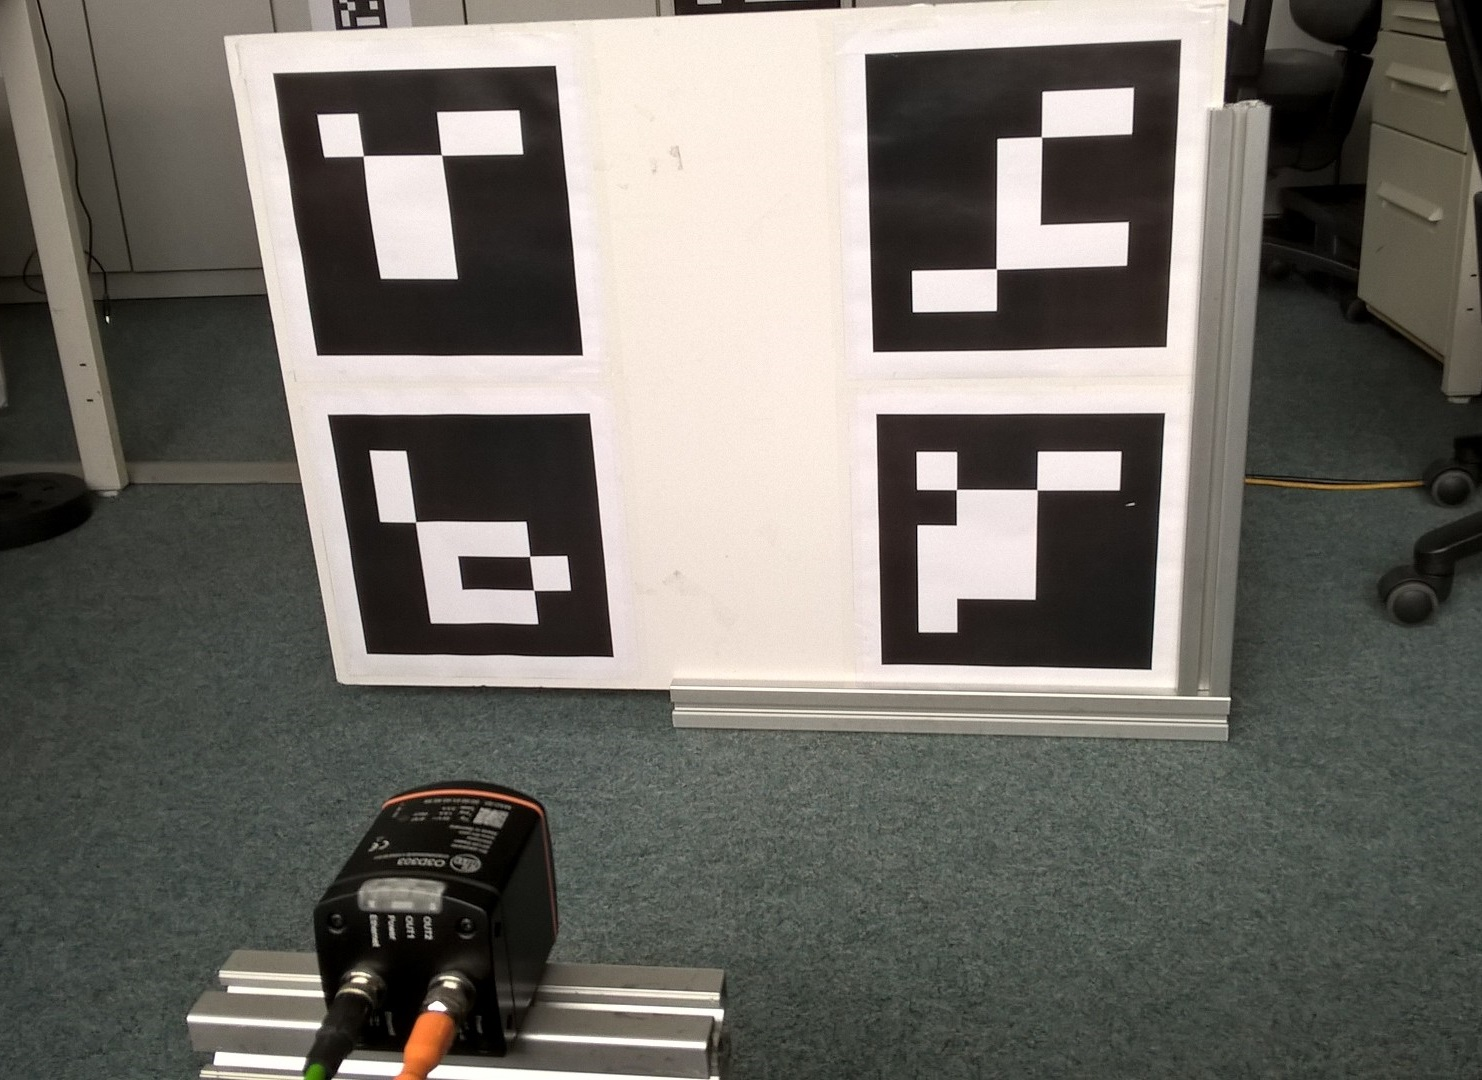
\includegraphics[width=.95\linewidth]{evaluation/ArUco_Foto}
    \caption{Foto des Versuchsaufbaus}
    \label{fig:systematic_error_foto}
\end{subfigure}%
\begin{subfigure}{.49\textwidth}
    \centering
    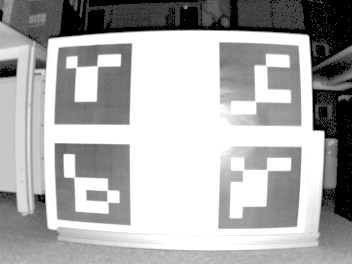
\includegraphics[width=.95\linewidth]{evaluation/ArUco_IR}
    \caption{Infrarotbild der O3D303}
    \label{fig:systematic_error_O3D303_ir}
\end{subfigure}
\caption{Versuchsaufbau zur Generierung von Ground Truth Tiefenwerten und resultierendes Infrarotbild der O3D303 während der Messung.}
\label{fig:systematoc_error_experiment}
\end{figure}

Der \emph{systematische Fehler}, in anderen Arbeiten oft auch als \emph{Wiggling Error} bezeichnet, wird dadurch verursacht, dass das emittierte amplitudenmodulierte Signal von einer perfekten Sinuswelle abweicht und die Schätzung der Phasenverschiebung daher einen Fehler in Abhängigkeit zur Distanz aufweist \cite{bib:Giancola2018}. Zur Messung des distanzabhängigen Fehlers wird eine Ground Truth Distanz benötigt, mit der die gemessene Distanz des Sensors verglichen werden kann. Giancola et al. \cite{bib:Giancola2018} verwendeten in ihrer Arbeit einen Roboterarm, der extrinsisch auf die Kamera kalibriert wurde, wodurch die Distanz zwischen Roboterarm und Sensor bekannt war. Diese Arbeit verwendet ArUco Marker zur Ermittlung der Ground Truth Distanz zwischen der Messfläche und dem Sensor. Bei ArUco handelt es sich um eine Bibliothek für \emph{Augmented Reality} Anwendungen, die an der Córdoba Universität entwickelt wurde \cite{bib:Ramirez2018}\cite{bib:Garrido-Jurado2015}. Mittels ArUco ist es möglich Marker im Bild zu erkennen und die Position und Orientierung relativ zur Kamera zu bestimmen. Wenn die ArUco Marker auf einer planaren Oberfläche angebracht werden, ist es möglich die Entfernung der Messfläche, die sich zwischen den vier ArUco Markern befindet, zur Kamera zu approximieren. Für die Aufnahme wurde die Kamera fixiert und die Messfläche orthogonal zur optischen Achse ausgerichtet, wobei die Entfernung der Messfläche zur Kamera langsam erhöht wurde. \autoref{fig:systematic_error_foto} zeigt den Versuchsaufbau, mit dem die Daten für die O3D303 erhoben wurden. 

Da die Auflösung des Bildes zur genauen Bestimmung der Position der ArUco Marker eine wichtige Rolle spielt, wurden für die Xtion 2 und die Kinect v2 die Farbbildkamera zur Bestimmung der Markerpositionen verwendet, da diese über eine höhere Auflösung verfügen. Die Tiefenbildkamera und die Farbbildkamera wurden mit Hilfe eines Schachbrettmusters extrinsisch aufeinander kalibriert und die berechneten Tiefeninformationen aus dem Farbbild wurden anschließend in den Raum des Tiefenbildes transformiert. Allerdings führt die Bestimmung der Markerposition einen eigenen Fehler mit sich, der mit zunehmender Enfernung zum Marker größer wird und sich durch einem Rauschverhalten in den Aufnahmen äußert, da die Bestimmung der Ecken der Marker ungenauer wird.

\begin{figure}[hp!]
\centering
\begin{subfigure}{\textwidth}
\begin{tikzpicture}
\begin{axis}[
    width=\textwidth, 
    height=\axisdefaultheight,
    xlabel={Tatsächlicher Tiefenwert in mm},
    ylabel={Abweichung des Tiefenwerts in mm},
    xmin=700, xmax=3000,
    ymin=-20, ymax=0,
    xtick={700,1000,1500,2000,2500,3000},
    ytick={-20,-15,-10,-5,0},
    legend pos=south east,
    ymajorgrids=true,
    grid style=dashed,
]

\addplot+[ 
    color=blue,
    only marks,
    mark=*,
    mark size=0.5pt
    ]
    table {../graphs/systematic_error_kinect_raw.dat};
\addlegendentry{Kinect v2}
\end{axis}
\end{tikzpicture}
\end{subfigure}

\begin{subfigure}{\textwidth}
\centering
\begin{tikzpicture}
\begin{axis}[
    width=\textwidth, 
    height=\axisdefaultheight,
    xlabel={Tatsächlicher Tiefenwert in mm},
    ylabel={Abweichung des Tiefenwerts in mm},
    xmin=700, xmax=3000,
    ymin=-90, ymax=30,
    xtick={700,1000,1500,2000,2500,3000},
    ytick={-90,-80,-70,-60,-50,-40,-30,-20,-10,0,10,20,30,40,50},
    legend pos=south east,
    ymajorgrids=true,
    grid style=dashed,
]

\addplot+[ 
    color=red,
    only marks,
    mark=*,
    mark size=0.5pt
    ]
    table {../graphs/systematic_error_xtion_raw.dat};
\addlegendentry{Xtion 2}
\end{axis}
\end{tikzpicture}
\end{subfigure}

\begin{subfigure}{\textwidth}
\centering
\begin{tikzpicture}
\begin{axis}[
    width=\textwidth, 
    height=\axisdefaultheight,
    xlabel={Tatsächlicher Tiefenwert in mm},
    ylabel={Abweichung des Tiefenwerts in mm},
    xmin=700, xmax=3000,
    ymin=-100, ymax=0,
    xtick={700,1000,1500,2000,2500,3000},
    ytick={-90,-80,-70,-60,-50,-40,-30,-20,-10,0},
    legend pos=south east,
    ymajorgrids=true,
    grid style=dashed,
]

\addplot+[ 
    color=black,
    only marks,
    mark=*,
    mark size=0.5pt
    ]
    table {../graphs/systematic_error_o3d303_raw.dat};
\addlegendentry{O3D303}
\end{axis}
\end{tikzpicture}
\end{subfigure}

\caption{Systematischer Fehler bei der Messung der Tiefenwerte in Abgängigkeit zur tatsächlichen Distanz.}
\label{fig:wiggle_error}
\end{figure}

Die \autoref{fig:wiggle_error} zeigt das Ergebnis der Messungen. Es ist dazu anzumerken, dass die O3D303 über keine Farbbildkamera verfügt und die Auflösung der Infrarotbildkamera mit 352 x 264 zu gering ausfällt, um eine genaue Bestimmung der ArUco Markerpositionen im Bild zu garantieren. Daher wurden drei Aufnahmen mit unterschiedlichen Markergrößen überlagert, um eine angemessene Genauigkeit zu ermöglichen, wodurch aber auch Fehler in die Messung eingeführt wurden. Die Ergebnisse der Kinect v2 decken sich mit den Messergebnissen von Giancola et al. \cite{bib:Giancola2018}, die eine Überlagerung mehrerer Sinuswellen feststellten. Giancola et al. \cite{bib:Giancola2018} und Keller \cite{bib:Keller2015} bestimmten mit Hilfe einer Fourier-Transformation zusätzlich die Phase und Amplitude der Sinuswellen, welche von Keller \cite{bib:Keller2015} zur Simulation des Fehlers genutzt wurden, worauf im Rahmen dieser Arbeit verzichtet wird. Die Messergebnisse der O3D303 lassen darauf schließen, dass es sich bei dem Verlauf der Abweichung, ähnlich zu den Ergebnissen der Arbeit von Keller \cite{bib:Keller2015}, um nur eine Sinuswelle handeln könnte, da die O3D303 im Gegensatz zur Kinect v2 zur Generierung des Tiefenbildes nur eine Wellenfunktion mit einer Frequenz von 30 Mhz verwendet. Lediglich die Messwerte der Xtion 2 weichen von den Erwartungen ab, da keine Sinuswelle in den Messergebnissen ausgemacht werden kann.
%
\subsection{Multiple Path Fehler durch Indirekte Beleuchtung}\label{sec:multipath_problem}
%
\begin{figure}[h!]
\centering
\begin{subfigure}[b]{0.49\textwidth}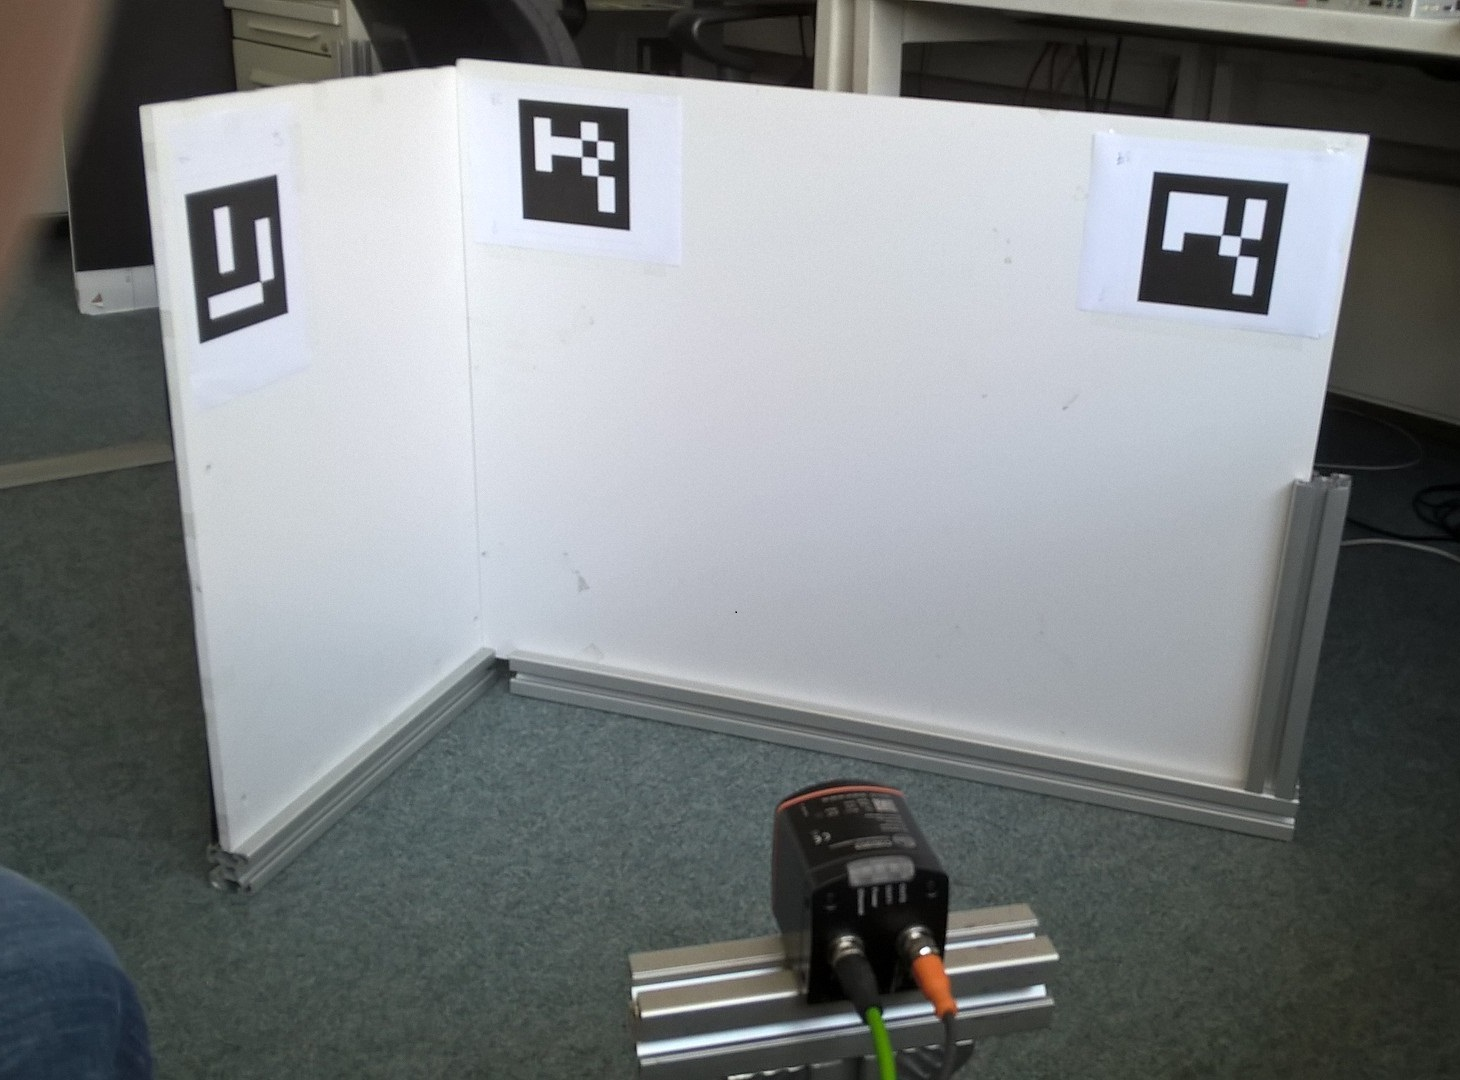
\includegraphics[width=\textwidth]{evaluation/Multiple_Path_Foto}
    \caption{Versuchsaufbau zur Multiple Path Fehler Messung}
\end{subfigure}
\begin{subfigure}[b]{0.49\textwidth}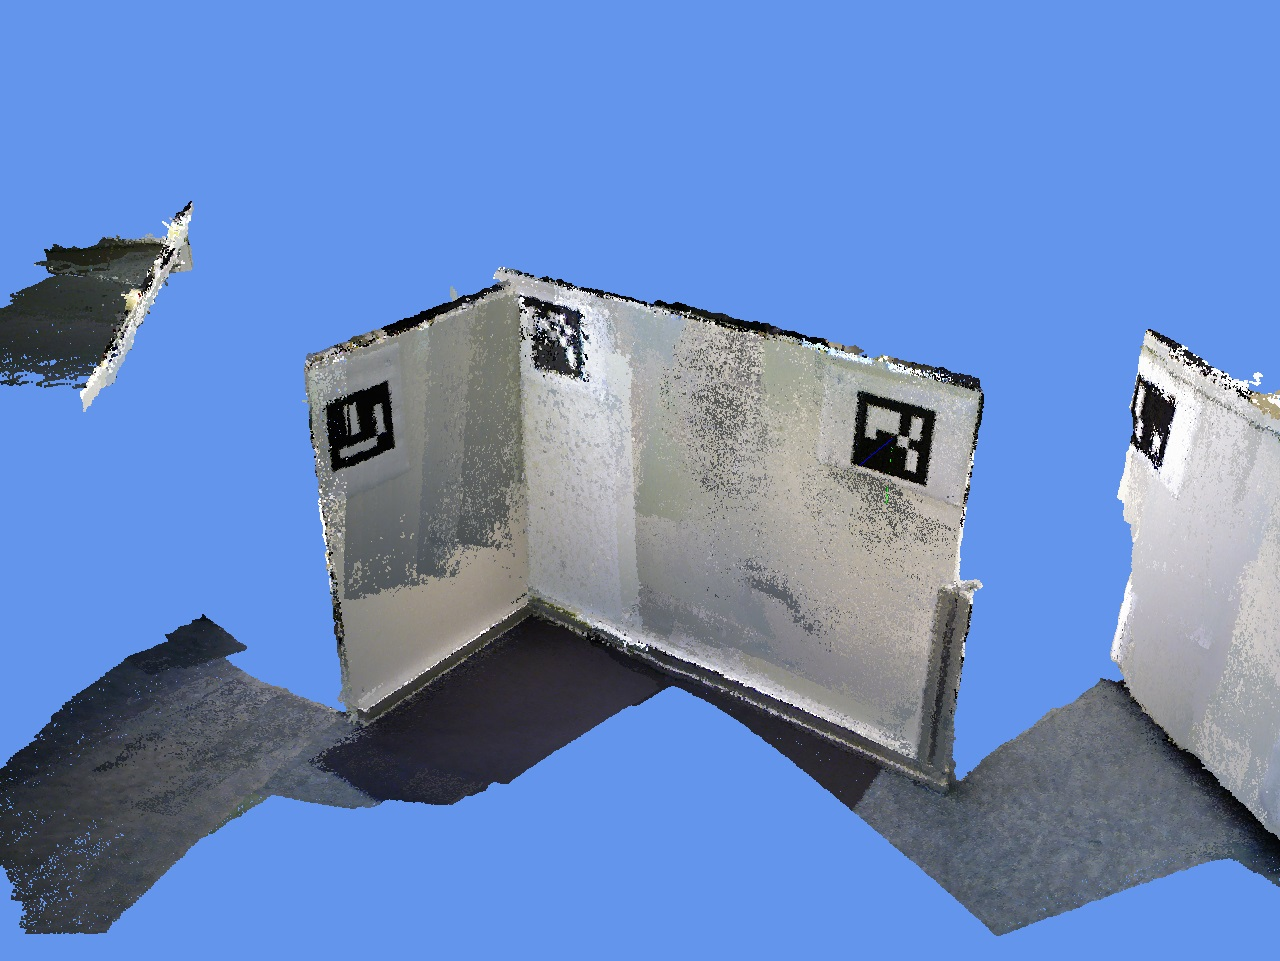
\includegraphics[width=\textwidth]{evaluation/Multiple_Path_PointCloud}
    \caption{Punktewolke des Versuchsaufbaus zur Bestimmung der Ground Truth Tiefenwerte}
\end{subfigure}
\caption{Versuchsaufbau mit orthogonal angeordneten Flächen zur Messung des Multipath Fehlers und die Punktewolke des Versuchsaufbaus, die als Referenz verwendet wurde.}
\label{fig:multiple_path_error_experiment}
\end{figure}

Bei dem \emph{Multipath Fehler} handelt es sich um einen Fehler bei der Berechnung der Tiefenwerte, der durch den Einfluss von indirekter Beleuchtung verursacht wird. Durch Reflexionen an der Oberfläche wird das emittierte Licht über Umwege zum Sensor reflektiert. Dies führt zu einer höheren Schätzung des Tiefenwerts, da indirekte Reflexionen einen längeren Weg zurückgelegt haben als direkte Reflexionen, bevor sie zum Sensor gelangen. Für die Untersuchung des Einflusses der indirekten Beleuchtung wurden für den Versuchsaufbau zwei helle Platten orthogonal zueinander vor der Kamera aufgebaut an denen jeweils ArUco Marker angebracht sind, um die Kameraposition in Relation zu den Flächen bestimmen zu können. 

Um die Tiefenwerte, die vom Tiefensensor geliefert werden mit Ground Truth Tiefenwerten vergleichen zu können, wurde eine Punktewolke des Versuchsaufbaus mit einer \emph{Structured Light} Kamera generiert. Bei einer Structured Light Kamera handelt es sich um ein Kamerasystem, das mit einem Infrarotprojektor ein bekanntes Punktmuster projiziert, welches mit einer Infrarotkamera erfasst wird, woraus Tiefenwerte generiert werden. Bei dem Verfahren handelt es sich um ein von PrimeSense entwickeltes proprietäres Verfahren, weshalb nicht im Detail auf die Funktionsweise eingegangen werden kann.

\begin{figure}[h!]
\centering
\begin{subfigure}[b]{0.98\textwidth}
    \centering
    \includepdftex{scala_0_to_100}
\end{subfigure}
\vspace{5mm}
\begin{subfigure}[b]{0.32\textwidth}
    \includegraphics[width=\textwidth]{evaluation/Kinect_v2/multi_path_error_jetmap}
    \caption{Microsoft Kinect v2}
\end{subfigure}
\begin{subfigure}[b]{0.32\textwidth}
    \includegraphics[width=\textwidth]{evaluation/Xtion_2/multi_path_error_jetmap}
    \caption{ASUS Xtion 2}
\end{subfigure}
\begin{subfigure}[b]{0.32\textwidth}
    \includegraphics[width=\textwidth]{evaluation/O3D303/multi_path_error_jetmap}
    \caption{IFM O3D303}
\end{subfigure}
\caption{Multiple Path Fehler, der durch indirekte Beleuchtung der Flächen verursacht wird.}
\label{fig:multiple_path_error_evaluation}
\end{figure}

Die verwendete Xtion 1 Kamera weist keinen Multipath Fehler auf, weshalb sie zur Generierung von Ground Truth Tiefenwerten für dieses Experiment geeignet ist \cite{bib:Wasenmueller2017}. Die Xtion 1 weist zwar ebenfalls einen systematischen Fehler auf, dieser nimmt allerdings linear mit der gemessenen Entfernung zu und ist daher auf kurze Distanzen von bis zu 1000 mm ausreichend genau \cite{bib:Giancola2018}\cite{bib:Teichman2013}. Für die Generierung der Punktewolke fand außerdem das von Muñoz-Salinas et al. \cite{bib:Munoz-Salinas2017} entwickelte \emph{Marker Mapping} Verwendung. Mittels des Marker Mappings ließen sich die relativen Markerpositionen zueinander berechnen und in Form einer Marker Map nutzen, wodurch es möglich war bei der Generierung der Punktewolke für jeden ArUco Marker eine eindeutige Position im Raum zu bestimmen. Die Xtion 1 verfügt wie die Xtion 2 und die Kinect v2 über eine Farbbild- und eine Tiefenkamera, wodurch es möglich ist das Farbbild in Kombination mit der ArUco Marker Map zu nutzen, um die Orientierung der Kamera im Raum zu bestimmen und die gemessenen Tiefenwerte der Kamera entsprechend in den Raum zu transformieren. Die \autoref{fig:multiple_path_error_experiment} zeigt den Versuchsaufbau mit der O3D303 und die generierte Punktewolke, die zur Referenz verwendet wurde.

\begin{figure}[h!]
\centering
\begin{subfigure}{0.32\textwidth}
\begin{tikzpicture}
\begin{axis}[
    width=1.3\textwidth, 
    height=\axisdefaultheight,
    xmin=-475, xmax=475,
    ymin=350, ymax=1500,
    xtick={-1000},
    ytick={0},
    legend pos=north west,
    ymajorgrids=true,
    grid style=dashed,
]

\addplot+[ 
    color=red,
    mark=none
    ]
    table {../graphs/multi_path_error_kinect_depth.dat};

\addplot+[ 
    color=blue,
    mark=none
    ]
    table [ref] {../graphs/multi_path_error_kinect_ref.dat};
\end{axis}
\end{tikzpicture}
\caption{Kinect v2}
\end{subfigure}
\begin{subfigure}{0.32\textwidth}
\begin{tikzpicture}
\begin{axis}[
    width=1.3\textwidth, 
    height=\axisdefaultheight,
    xmin=-475, xmax=475,
    ymin=350, ymax=1500,
    xtick={-1000},
    ytick={0},
    legend pos=north west,
    ymajorgrids=true,
    grid style=dashed,
]

\addplot+[ 
    color=red,
    mark=none
    ]
    table {../graphs/multi_path_error_xtion_depth.dat};

\addplot+[ 
    color=blue,
    mark=none
    ]
    table [ref] {../graphs/multi_path_error_xtion_ref.dat};
\end{axis}
\end{tikzpicture}
\caption{Xtion 2}
\end{subfigure}
\begin{subfigure}{0.32\textwidth}
\begin{tikzpicture}
\begin{axis}[
    width=1.3\textwidth, 
    height=\axisdefaultheight,
    xmin=-475, xmax=475,
    ymin=350, ymax=1500,
    xtick={-1000},
    ytick={0},
    legend pos=north west,
    ymajorgrids=true,
    grid style=dashed,
]

\addplot+[ 
    color=red,
    mark=none
    ]
    table {../graphs/multi_path_error_o3d303_depth.dat};

\addplot+[ 
    color=blue,
    mark=none
    ]
    table [ref] {../graphs/multi_path_error_o3d303_ref.dat};
\end{axis}
\end{tikzpicture}
\caption{O3D303}
\end{subfigure}
\caption{Top-Down Darstellung der Tiefenwerte aus dem mittleren horizontalen Schnitt des Bildes. Die blauen Tiefenwerte stehen für die Ground Truth Distanz und die roten Tiefenwerte repräsentieren die Messwerte der einzelnen Kameras.}
\label{fig:multiple_path_error_evaluation_depth}
\end{figure}

Für jede Kamera wurden 10000 Tiefenbilder der statischen Szene aufgenommen und für jeden Pixel wurde der durchschnittliche Tiefenwert gebildet, um den zufälligen Fehler, der in \autoref{sec:noise_error} erläutert wurde, zu reduzieren. Mit Hilfe der ArUco Marker wurde die Punktewolke so transformiert, dass sie mit den realen Positionen des Versuchsaufbaus relativ zur Kamera übereinstimmt. Dadurch konnte eine Abweichung der gemessenen Tiefenwerte zu den erwarteten Tiefenwerten festgestellt werden. \autoref{fig:multiple_path_error_evaluation} veranschaulicht das Ergebnis des Versuchs in Form einer Color Map. Dabei ist zu erkennen, dass sich die Einflüsse des Multipath Fehlers für jede Kamera im Detail unterscheiden, aber gemeinsam haben, dass Ecken im Bild durch den Einfluss von Interreflexionen abgerundet werden. \autoref{fig:multiple_path_error_evaluation_depth} stellt dieses Verhalten noch deutlicher dar, indem die Tiefenwerte der Punktewolke und der Time-of-Flight Kameras in der Mitte des Bildes entlang einer horizontalen Scanlinie verglichen werden. 
%
\subsection{Lens Scattering Fehler}\label{sec:lens_scattering}
%
\begin{figure}[h!]
\centering
\begin{subfigure}[b]{0.49\textwidth}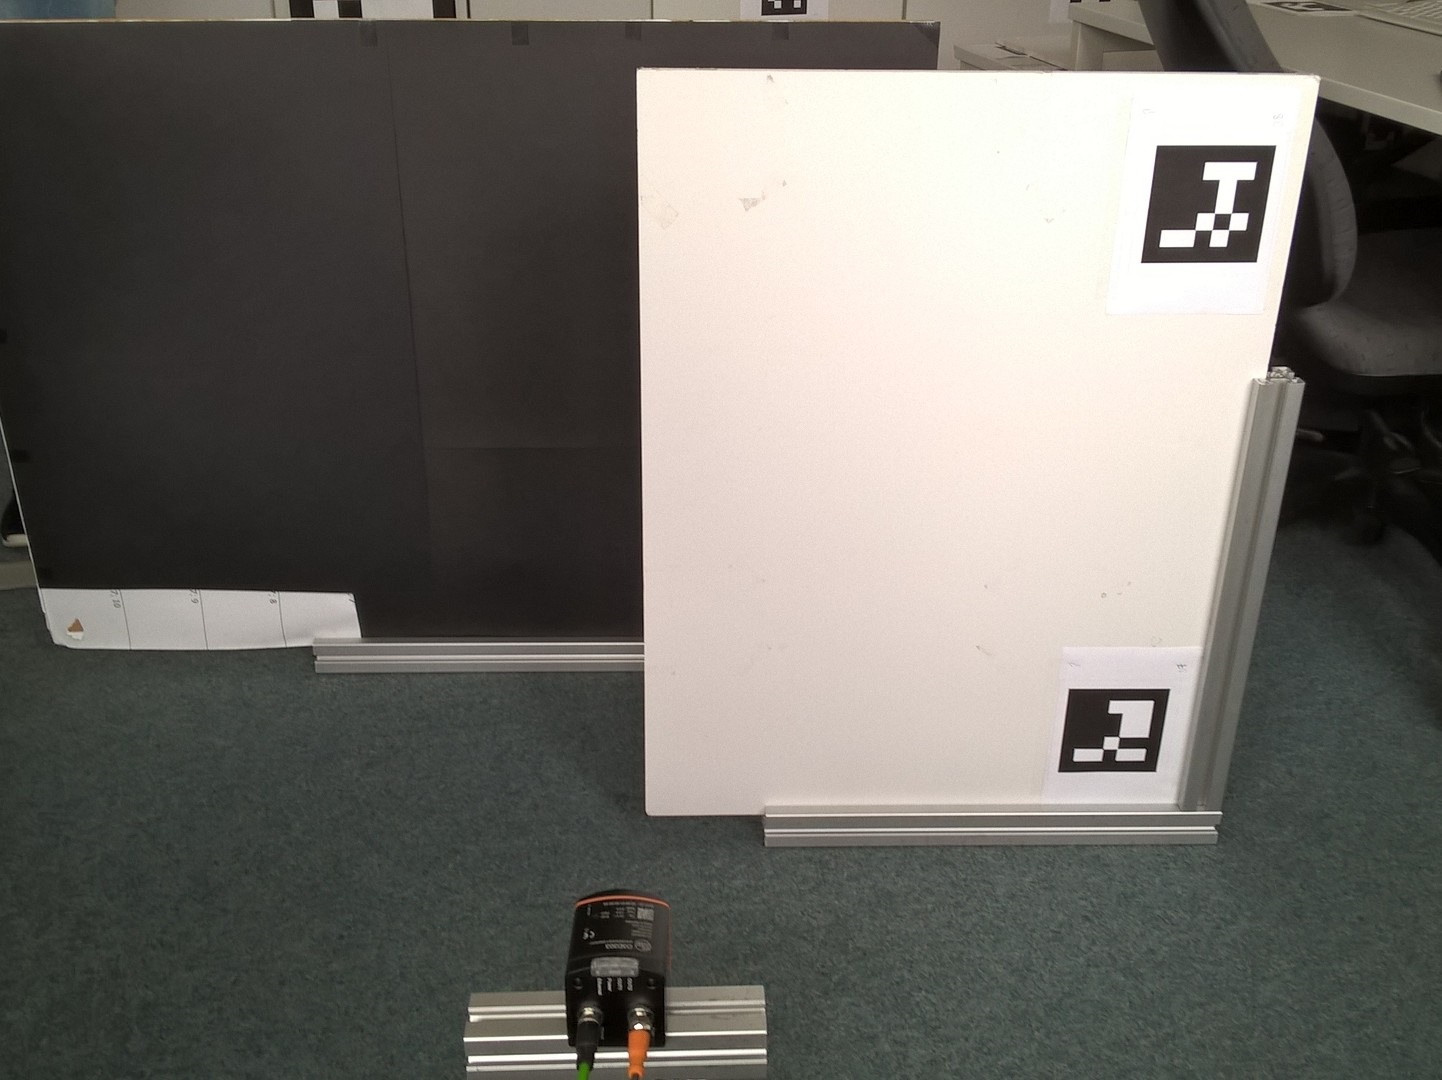
\includegraphics[width=\textwidth]{evaluation/Lens_Scattering_Experiment}
    \caption{Versuchsaufbau zur Messung des Lens Scattering Fehlers}
\end{subfigure}
\begin{subfigure}[b]{0.49\textwidth}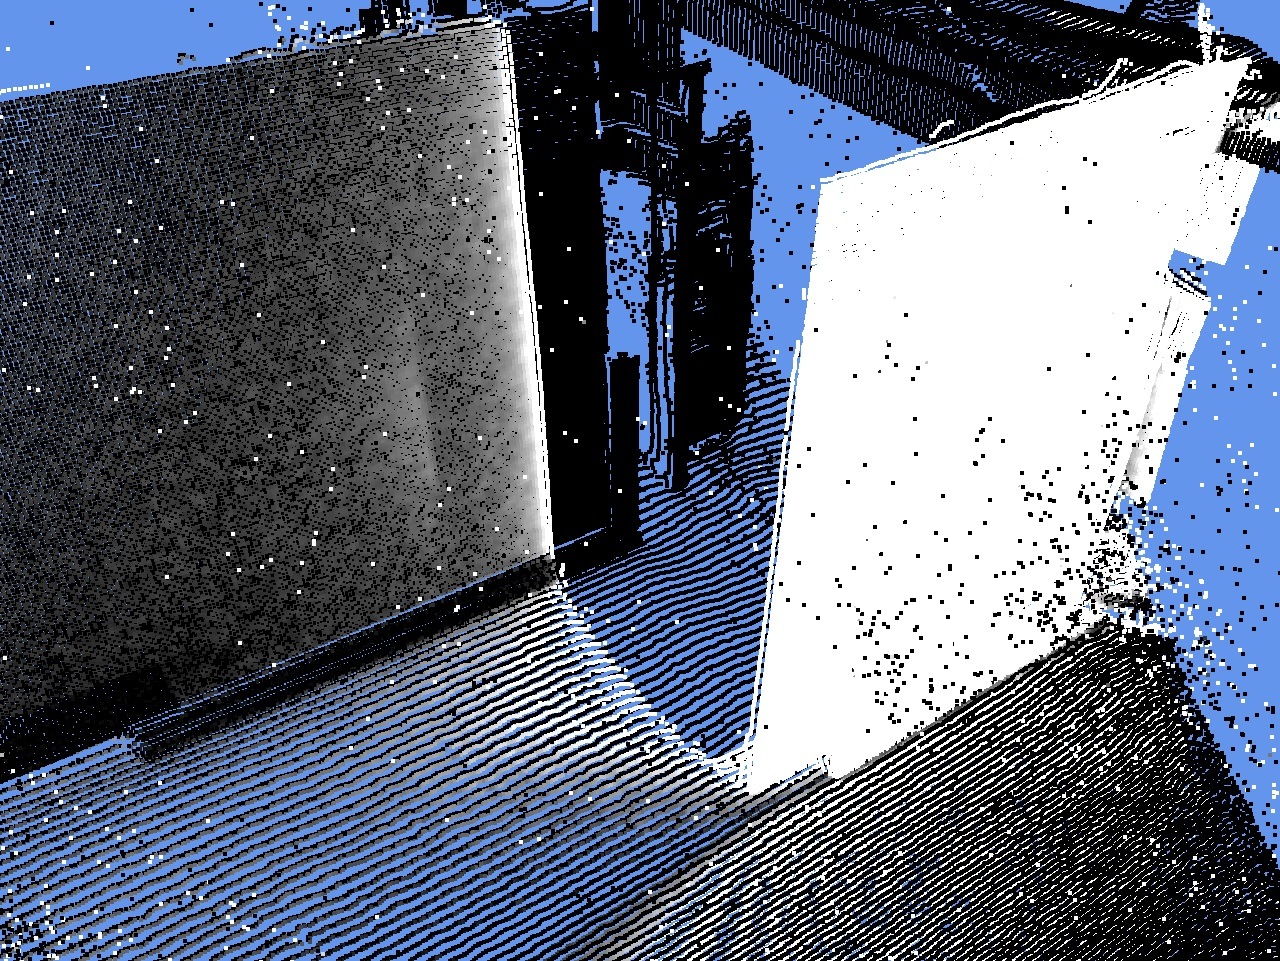
\includegraphics[width=\textwidth]{evaluation/Lens_Scattering_Point_Cloud}
    \caption{Punktewolke des Versuchsaufbaus mit resultierendem Lens Scattering Fehler}
\end{subfigure}
\caption{Versuchsaufbau zur Evaluierung des Lens Scattering Fehlers. Zu erkennen ist der Fehler an den hell eingefärbten Pixeln im Hintergrund, der direkt am Übergang stark ausgeprägt ist und mit größerer Entfernung zum Vordergrund abnimmt.}
\label{fig:lens_scattering_experiment}
\end{figure}

Der \emph{Lens Scattering Fehler} beschreibt einen aus der Literatur bekannten Fehler im Tiefenbild, der dadurch verursacht wird, dass das einfallende Licht einen Einfluss auf benachbarte Pixel ausübt \cite{bib:Hertzberg2014}\cite{bib:Jamtsho2010}\cite{bib:Mure-Dubois2007}\cite{bib:Mure-Dubois2009}. Zusätzlich zur Beugung durch die Blende werden Reflexionen und Streuungseffekte innerhalb des Linsensystems als Grund für verfälschte Tiefenwerte benachbarter Pixel genannt. Dieser auftretende Effekt verursacht, dass stark beleuchtete Objekte im Vordergrund die Tiefenwerte der Objekte beeinflussen, die sich im Hintergrund befinden und schwächer beleuchtet werden. Hertzberg und Frese \cite{bib:Hertzberg2014} untersuchten den Lens Scattering Effekt mit Hilfe eines runden Retroreflektors der vor einen schwach reflektierenden Hintergrund positioniert wurde. Dazu wurde zunächst eine Aufnahme des Hintergrundes ohne Reflektor erstellt und anschließend die selbe Szene mit Reflektor aufgenommen. Dadurch konnte der Einfluss des Retroreflektors auf den Hintergrund bestimmt werden. In dieser Arbeit wird von der Verwendung eines Retroreflektors abgesehen, da dieser neben dem Lens Scattering Effekt bei allen Sensoren zusätzlich \emph{Blendenflecke} oder \emph{Linsenreflexionen} verursacht hat. Zusätzlich führte die Verwendung des Retroreflektors dazu, dass die Intensität des Infrarotbildes des Reflektors gesättigt war und so die ursprüngliche Intensität der reflektierten Strahlung nicht mehr ermittelt werden konnte, was die Aufnahme für die Evaluation des Lens Scattering Effekts unbrauchbar macht. 

\begin{figure}[h!]
\centering
\begin{tikzpicture}
\begin{axis}[
    width=\textwidth, 
    height=\axisdefaultheight,
    xlabel={x-Koordinate},
    ylabel={z-Koordinate},
    xmin=-500, xmax=500,
    ymin=700, ymax=1800,
    legend pos=north west,
    ymajorgrids=true,
    grid style=dashed,
]

\addplot+[ 
    color=red,
    mark=*,
    only marks,
    mark size=1.0pt
    ]
    table {../graphs/lens_scattering_error_o3d303_depth.dat};

\addplot+[ 
    color=blue,
    mark=*,
    only marks,
    mark size=1.0pt
    ]
    table [ref] {../graphs/lens_scattering_error_o3d303_ref.dat};
\end{axis}
\end{tikzpicture}
\caption{Top-Down Darstellung der Tiefenwerte aus dem mittleren horizontalen Schnitt des Bildes.}
\label{fig:lens_scattering_evaluation_one}
\end{figure}

Jamtsho und Lichti \cite{bib:Jamtsho2010} verwendeten zur Evaluation hingegen zwei stark reflektierende Flächen in unterschiedlichen Distanzen, die orthogonal zur optischen Achse des Sensors positioniert wurden. Dabei wurde der Einfluss der Tiefenwerte der Fläche, die sich näher am Sensor befindet, auf die Tiefenwerte der Fläche im Hintergrund beobachtet. Diese Arbeit verfolgt einen ähnlichen Ansatz und verwendet eine schwach reflektierende Fläche aus schwarzem Tonpapier im Hintergrund und eine stark reflektierende Fläche im Vordergrund. Dabei wird die Distanz der stark reflektierenden Fläche zur Kamera variiert und der Einfluss auf den Hintergrund beobachtet. \autoref{fig:lens_scattering_experiment} veranschaulicht den Versuchsaufbau und die resultierende Punktewolke der Messung, die im Folgenden im Detail untersucht wird.

\begin{figure}[h!]
\centering
\begin{subfigure}{0.49\textwidth}
\centering
\begin{tikzpicture}
\begin{axis}[
    width=\textwidth, 
    height=\axisdefaultheight,
    xmin=-10, xmax=10,
    ymin=-0.1, ymax=1.1,
    legend pos=north west,
    ymajorgrids=true,
    grid style=dashed,
]

\addplot+[smooth][ 
    color=red,
    mark=none
    ]
    table {../graphs/lens_scattering_o3d303.dat};
\end{axis}
\end{tikzpicture}
\caption{IFM O3D303}
\label{fig:lens_scattering_results_o3d393}
\end{subfigure}
\begin{subfigure}{0.49\textwidth}
\centering
\begin{tikzpicture}
\begin{axis}[
    width=\textwidth, 
    height=\axisdefaultheight,
    xmin=-10, xmax=10,
    ymin=-0.1, ymax=1.1,
    legend pos=north west,
    ymajorgrids=true,
    grid style=dashed,
]

\addplot+[smooth][ 
    color=red,
    mark=none
    ]
    table {../graphs/lens_scattering_kinect.dat};
\end{axis}
\end{tikzpicture}
\caption{Microsoft Kinect v2}
\label{fig:lens_scattering_results_kinect_v2}
\end{subfigure}
\caption{Lens Scattering Fehler in Abhängigkeit zur Intensität des Infrarotbildes.}
\label{fig:lens_scattering_results}
\end{figure}

In \autoref{fig:lens_scattering_evaluation_one} werden die Tiefenwerte aus der horizontalen Scanlinie dargestellt. Bei den blauen Tiefenwerten handelt es sich um die Referenzaufnahme des Hintergrundes. Die roten Tiefenwerte wurden einer Aufnahme entnommen, in der ein zusätzliches Objekt im Vordergrund des Bildes positioniert wurde. Der stark reflektierende Vordergrund beeinflusst dabei die Tiefenwerte der gesamten restlichen Aufnahme. An dem Übergang vom Vordergrund zum Hintergrund wirkt sich der Lens Scattering Fehler besonders auf die Tiefenwerte des Hintergrundes aus. Diese Beobachtungen decken sich ebenfalls mit denen von Hertzberg und Frese \cite{bib:Hertzberg2014} und Jamtsho und Lichti \cite{bib:Jamtsho2010}.

\autoref{fig:lens_scattering_results} zeigt das Ergebnis der Untersuchung des Lens Scattering Effekts. Die Graphen zeigen den Einfluss des Pixels auf seine Nachbarpixel in Abhängigkeit zur Intensität in Form einer Punktspreizfunktion. Diese gibt an, wie stark sich die Intensität eines Pixels auf seine Nachbarpixel verteilt. Die Ergebnisse weichen von denen der Untersuchungen durch Hertzberg und Frese \cite{bib:Hertzberg2014} und Jamtsho und Lichti \cite{bib:Jamtsho2010} ab. Während Hertzberg und Frese einen ausschließlich positiven Verlauf der Funktion ermittelt haben, weist hier die O3D303 ebenfalls negative Werte auf (siehe \autoref{fig:lens_scattering_results_o3d393}). Jamtsho und Lichti näherten die Lens Scattering Funktion mittels einer Summe von Gaußfunktionen an, was für die Ergebnisse der O3D303 und Kinect v2 nicht möglich ist, da die Funktion im positiven Bereich nicht monoton fallend und im negativen Bereich nicht monoton steigend ist. Der Funktionsverlauf erinnert dabei an den Verlauf von \emph{Beugungsscheibchen} oder auch \emph{Airy-Scheibchen} genannt, die durch die Beugung eines Lichtstrahls an einer Blende entstehen \cite{bib:Padley2009}, weshalb ein Zusammenhang vermutet wird.
%
\subsection{Mixed Pixels Fehler}\label{sec:mixed_pixels}
%
\begin{figure}[h!]
\centering
\begin{subfigure}[b]{0.49\textwidth}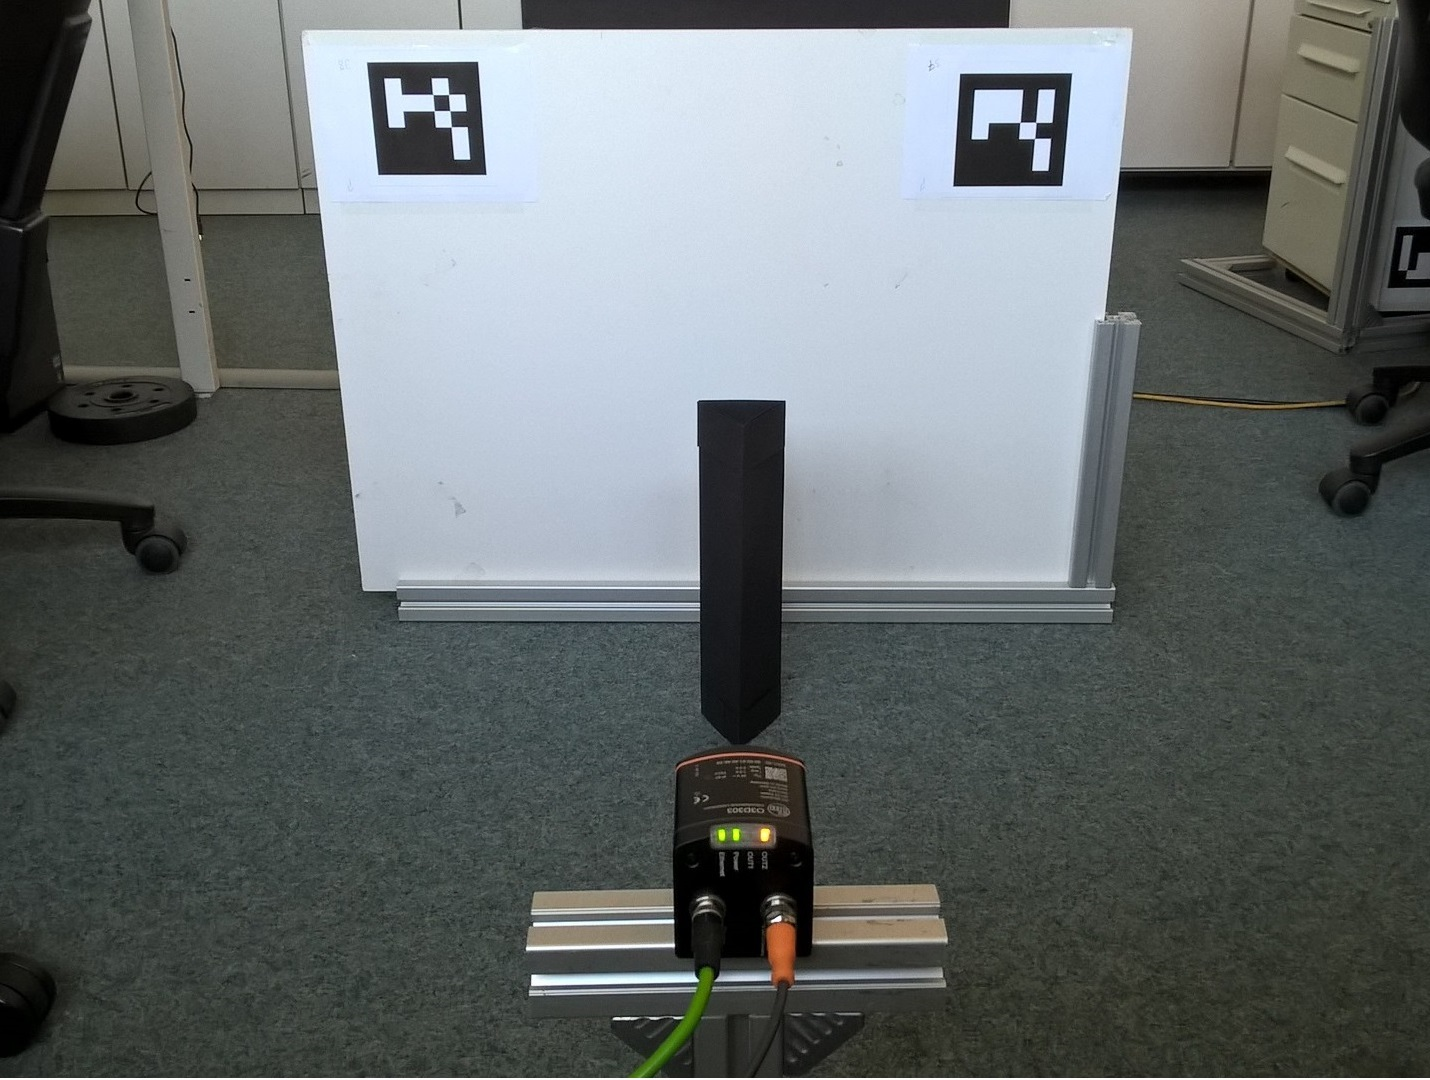
\includegraphics[width=\textwidth]{evaluation/Mixed_Pixels_Experiment}
    \caption{Versuchsaufbau zur Mixed Pixels Fehler Messung}
\end{subfigure}
\begin{subfigure}[b]{0.49\textwidth}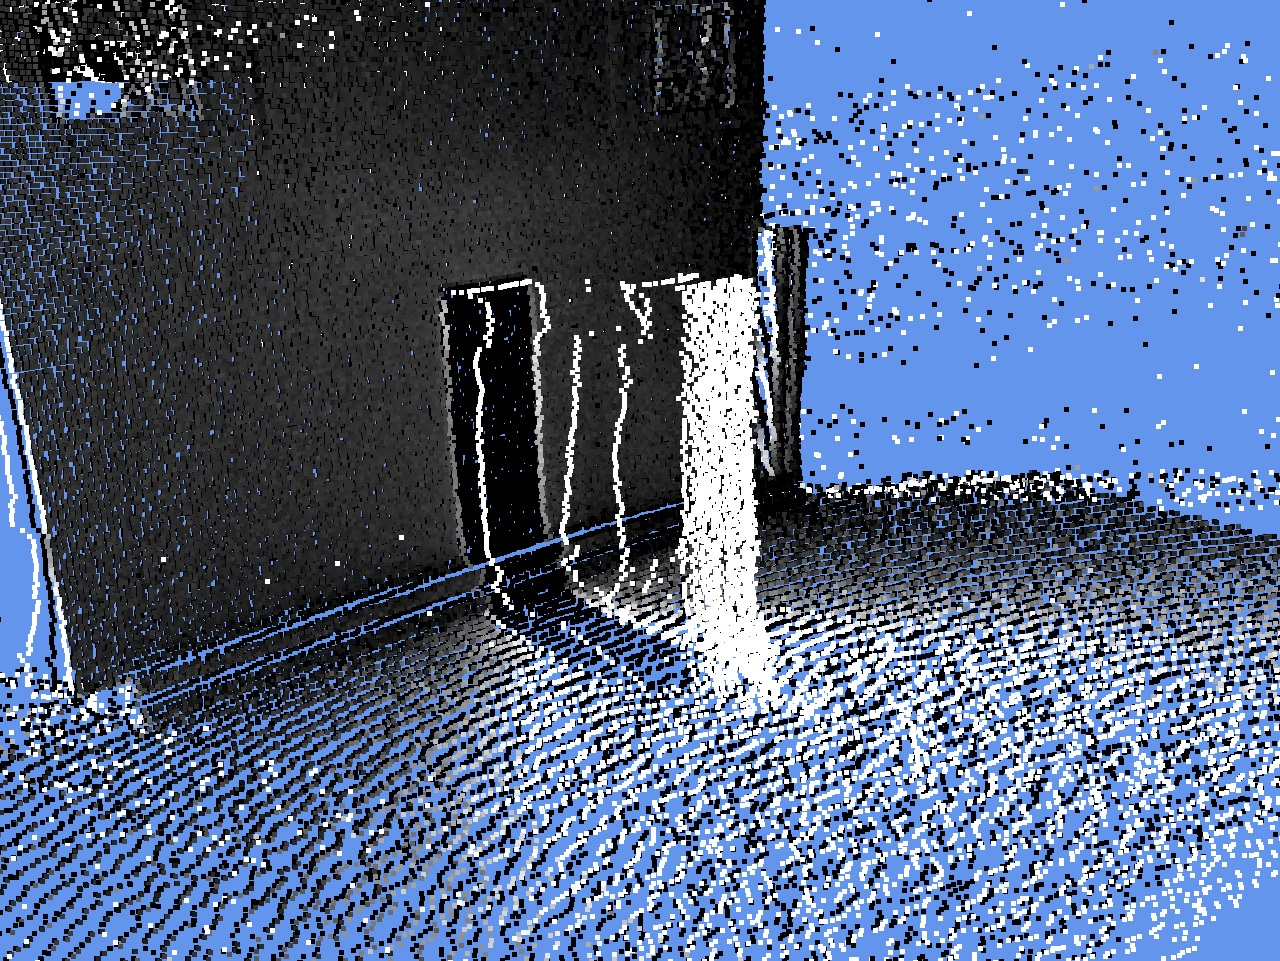
\includegraphics[width=\textwidth]{evaluation/Mixed_Pixels_PointCloud}
    \caption{Punktewolke des Versuchsaufbaus mit resultierendem Mixed Pixels Fehler}
\end{subfigure}
\caption{Versuchsaufbau zur Evaluierung des Mixed Pixels Fehler. Zu erkennen ist der Fehler an den fliegenden Punkten zwischen Vordergrundobjekt und Hintergrund.}
\label{fig:mixed_pixels_experiment}
\end{figure}

Der \emph{Mixed Pixels} Fehler, häufig auch \emph{Flying Pixels} Fehler genannt, beschreibt einen aus der Literatur bekannten Fehler im Tiefenbild, der an direkt benachbarten Tiefenwerten zu beobachten ist und der dadurch verursacht wird, dass sich ein Tiefenwert für einen Pixel aus mehreren gemessenen Tiefen zusammensetzt \cite{bib:Giancola2018}\cite{bib:Teichman2013}\cite{bib:Butkiewicz2014}\cite{bib:Hertzberg2014}. Dieser Fehler ist besonders in Bereichen mit stark variierenden Tiefenwerten zu beobachten. Da der Einfluss des Lens Scattering für die Evaluation des Mixed Pixels Fehlers ausgeschlossen werden muss, wird der Fehler zunächst isoliert, indem der Einfluss des Lens Scattering zunächst entfernt wird. Zur Evaluation des Mixed Pixels Fehlers wurde daher ein schwach reflektierendes Objekt vor einem stark reflektierenden Hintergrund positioniert und der Einfluss der schwach reflektierenden Oberfläche auf den Hintergrund wurde dabei beobachtet. Der Einfluss des Lens Scattering Effekts ist für diese Beobachtung nicht vollständig auszuschließen, allerdings sollte der Vordergrund einen verhältnismäßig geringen Einfluss auf den Hintergrund ausüben. Auf diese Weise kann der Mixed Pixels Fehler für den Hintergrund isoliert vom Lens Scattering Fehler betrachtet werden.

\begin{figure}[h!]
\centering
\begin{tikzpicture}
\begin{axis}[
    width=\textwidth, 
    height=\axisdefaultheight,
    xlabel={x-Koordinate},
    ylabel={z-Koordinate},
    xmin=-250, xmax=200,
    ymin=1000, ymax=1400,
    legend pos=north west,
    ymajorgrids=true,
    grid style=dashed,
]

\addplot+[ 
    color=red,
    mark=*,
    only marks,
    mark size=1.0pt
    ]
    table {../graphs/mixed_pixels_error_o3d303_depth.dat};

\addplot+[ 
    color=blue,
    mark=*,
    only marks,
    mark size=1.0pt
    ]
    table [ref] {../graphs/mixed_pixels_error_o3d303_ref.dat};
    
\addplot+[ 
    color=black,
    mark=*,
    only marks, 
    mark size=1.0pt
    ]
    table [ref] {../graphs/mixed_pixels_error_o3d303_test.dat};
\end{axis}
\end{tikzpicture}
\caption{Top-Down Darstellung der Tiefenwerte aus dem mittleren horizontalen Schnitt des Bildes.}
\label{fig:mixed_pixels_evaluation_one}
\end{figure}

Zur Evaluation wurden mit der O3D303 drei separate Aufnahmen angefertigt. Zunächst wurde nur der Hintergrund aufgenommen, um den Einfluss des Vordergrundobjektes auf den Hintergrund zu evaluieren. Dabei wurden 10.000 Tiefenbilder erstellt und für jeden Pixel der Durchschnitt des Tiefenwertes gebildet, um den zufälligen Fehler zu eliminieren. Anschließend wurde ein Objekt vor dem Hintergrund platziert und auf dieselbe Weise eine weitere Aufnahme erstellt. Abschließend wurde der Hintergrund wieder entfernt und eine Aufnahme vom Vordergrundobjekt gemacht, um den Einfluss des Hintergrundes auf den Vordergrund zu evaluieren. In \autoref{fig:mixed_pixels_evaluation_one} werden die aus den Aufnahmen resultierenden Tiefenwerte aus der horizontalen Scanlinie des Tiefenbildes dargestellt. Die blauen Tiefenwerte stehen für den separat aufgenommenen Hintergrund, die schwarzen Tiefenwerte sind durch eine separate Aufnahme des Vordergrundobjektes entstanden und die roten Tiefenwerte bilden die gemeinsame Aufnahme von Vordergrund und Hintergrund. Dabei ist zu erkennen, dass das Vordergrundobjekt die Tiefenwerte des Hintergrundes kaum beeinflusst, auf der anderen Seite werden aber die Tiefenwerte des Vordergrundobjektes durch den Hintergrund verfälscht. Um den Einfluss des in \autoref{sec:lens_scattering} betrachteten Lens Scattering auszuschließen, wurden daher alle Tiefenwerte, die zum Vordergrund gehören maskiert.

\begin{figure}[h!]
\centering
\begin{tikzpicture}
\begin{axis}[
    width=\textwidth, 
    height=\axisdefaultheight,
    xlabel={x-Koordinate},
    ylabel={z-Koordinate},
    xmin=-250, xmax=200,
    ymin=1000, ymax=1400,
    legend pos=north west,
    ymajorgrids=true,
    grid style=dashed,
]

\addplot+[ 
    color=red,
    mark=*,
    only marks,
    mark size=1.0pt
    ]
    table [ref] {../graphs/mixed_pixels_error_o3d303_cleaned_background.dat};
    
\addplot+[ 
    color=black,
    mark=*,
    only marks, 
    mark size=1.0pt
    ]
    table [ref] {../graphs/mixed_pixels_error_o3d303_cleaned_foreground.dat};
\end{axis}
\end{tikzpicture}
\caption{Top-Down Darstellung der Tiefenwerte aus dem mittleren horizontalen Schnitt des Bildes. Dabei wurden alle Tiefenwerte aus der roten Punktewolke entfernt, von denen sicher ist, dass diese zum Vordergrundobjekt gehören.}
\label{fig:mixed_pixels_evaluation_two}
\end{figure}

Die \autoref{fig:mixed_pixels_evaluation_two} zeigt die gemeinsame Aufnahme des Vordergrundobjektes und des Hintergrundes, wobei die Tiefenwerte der gemeinsamen Aufnahme so modifiziert wurden, dass die Punkte entfernt wurden, die durch die separate Aufnahme des Vordergrundobjektes als Teil des Vordergrundes identifiziert wurden. Dabei ist zu erkennen, dass der Mixed Pixels Fehler fast vollständig verschwunden ist. Daher liegt die Vermutung nahe, dass der aus der Literatur bekannte Mixed Pixels Fehler allein auf den Lens Scattering Effekt zurückzuführen ist, da der Fehler bei dem Versuch der isolierten Betrachtung verschwindet.
%
\subsection{Positionen der Infrarot LEDs}\label{sec:analysis_led_position}
%
\begin{figure}[h!]
\centering
\begin{subfigure}[b]{0.49\textwidth}
    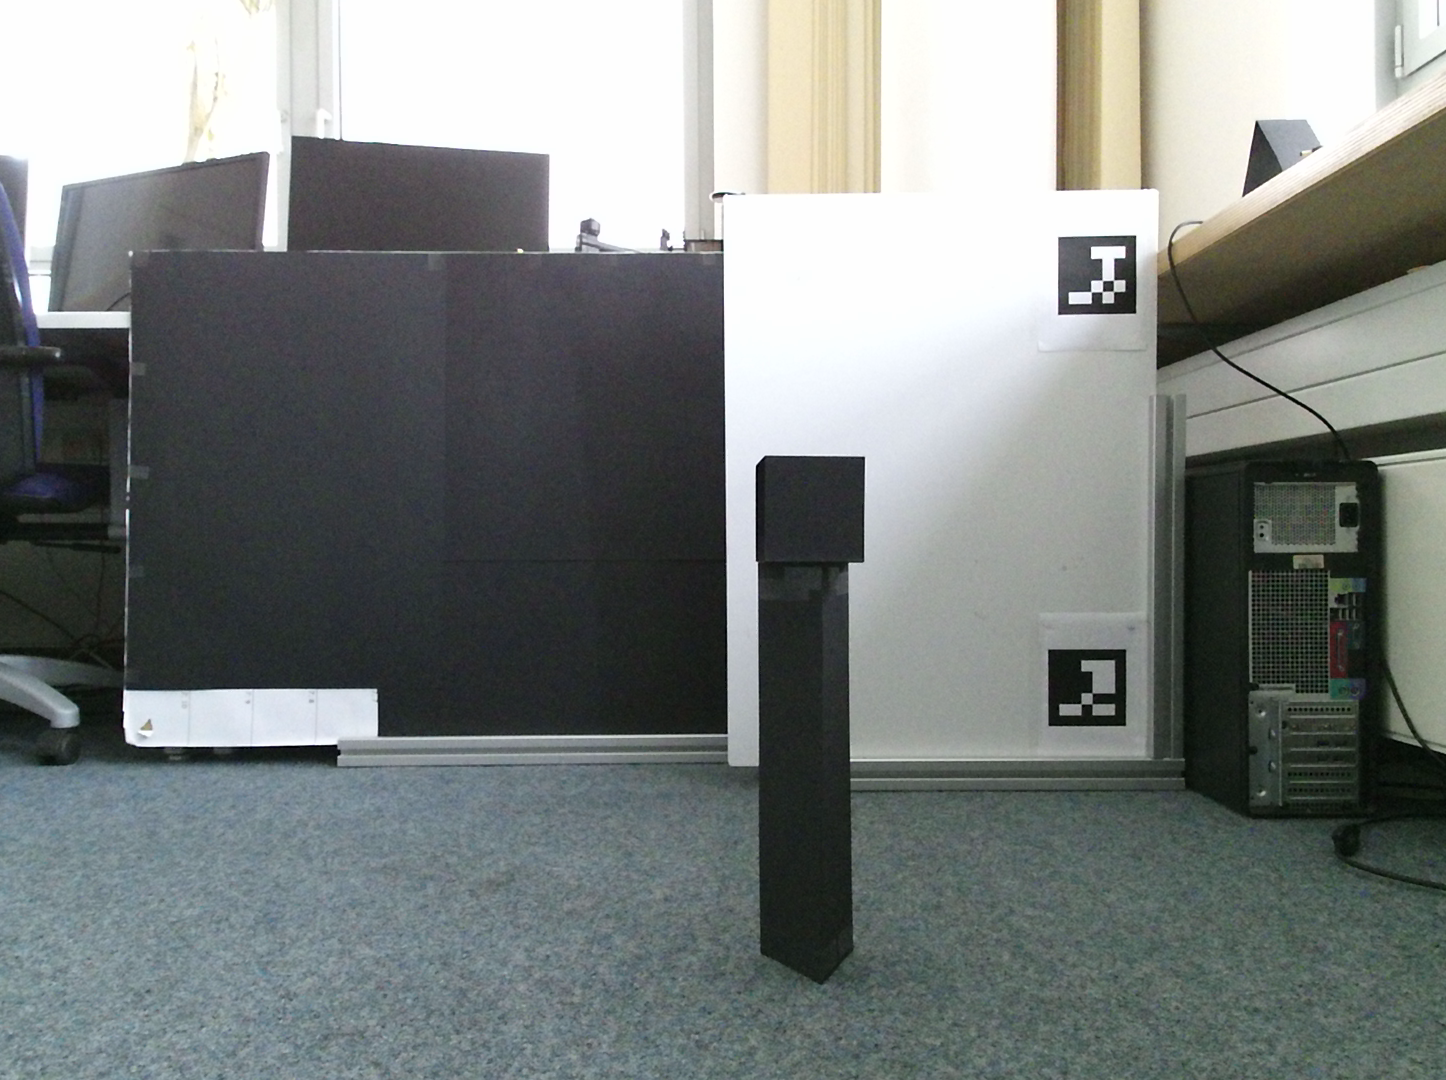
\includegraphics[width=\textwidth]{evaluation/shadow_error_rgb}
    \caption{Versuchsaufbau zur Messung des Fehlers durch Schattenwurf im Infrarotbild}
\end{subfigure}
\begin{subfigure}[b]{0.49\textwidth}
    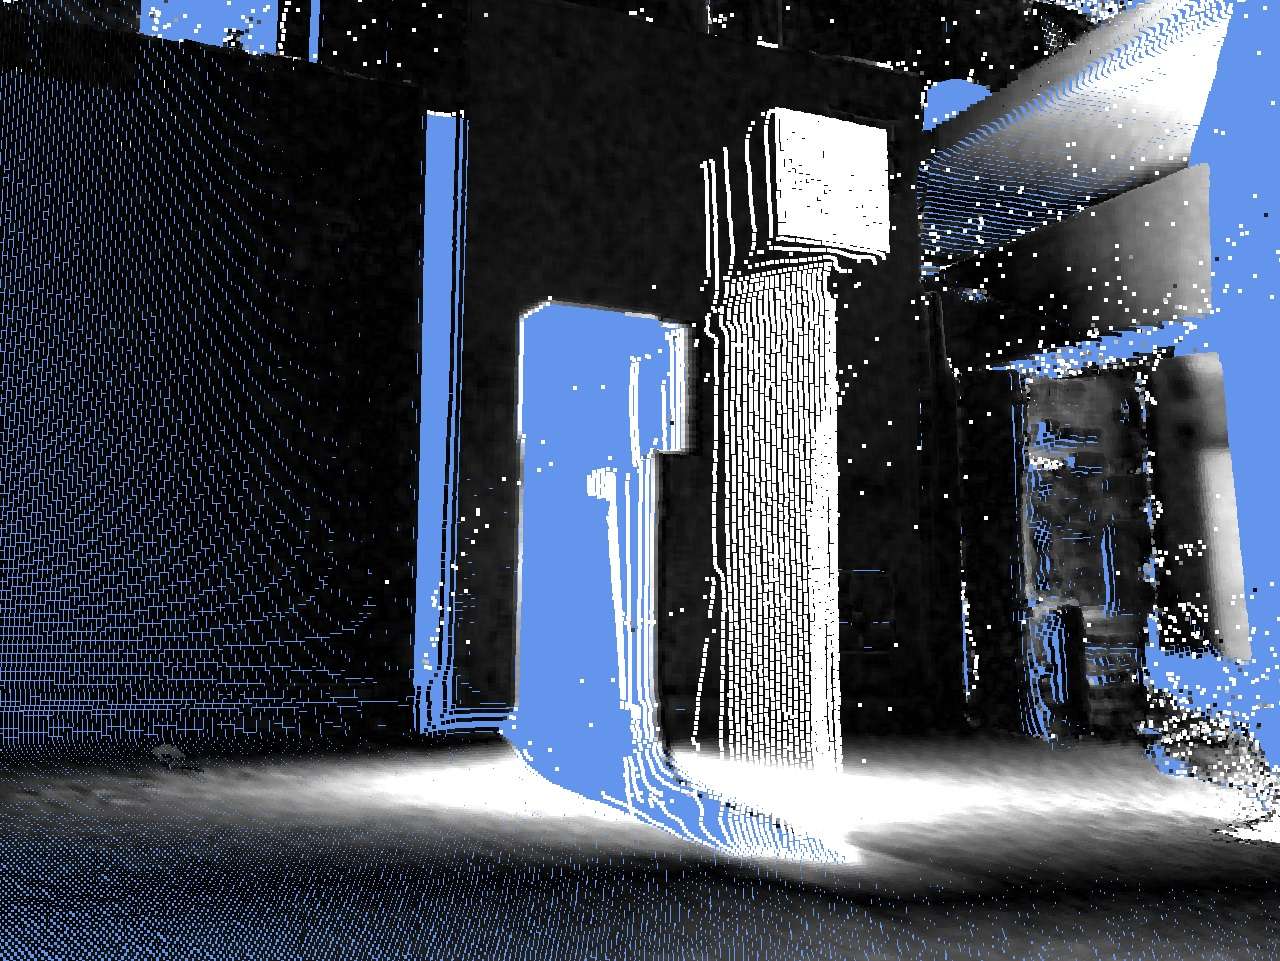
\includegraphics[width=\textwidth]{evaluation/shadow_error_pointcloud}
    \caption{Punktewolke des Versuchsaufbaus mit resultierendem Fehler}
\end{subfigure}
\caption{Versuchsaufbau zur Evaluierung des Fehlers durch Schatten. Zu erkennen ist der Fehler an den weißen Punkten im Hintergrund, dessen Tiefe zu hoch geschätzt wurde.}
\label{fig:shadow_error_experiment}
\end{figure}

Bei der Analyse des Mixed Pixels Fehlers ist aufgefallen, dass im Falle der Kinect v2 und der Xtion 2 ein Teil des Bildes im Schatten liegt und nicht direkt von den Infrarot LEDs bestrahlt wurde, wodurch Artefakte im Bild entstanden sind. Diese treten bei der O3D303 nicht auf, da der Sensor von vier LEDs umgeben ist. Die LEDs der Kinect v2 und der Xtion 2 sind einseitig neben dem Sensor positioniert, wodurch sich Schatten bilden können und Bildbereiche ausschließlich indirekt beleuchtet werden, was zu einer höheren Schätzung der Distanz führt.

Zur Untersuchung des Fehlers wurde zunächst eine Referenzaufnahme eines Hintergrundes  angefertigt. Anschließend wurde ein Objekt im Vordergrund positioniert und eine zweite Aufnahme angefertigt. Anschließend wurden die Aufnahmen miteinander verglichen und die Abweichung vom Referenzbild ermittelt. \autoref{fig:shadow_error_experiment} zeigt  den Versuchsaufbau und die resultierende Punktewolke. Dabei werden die Abweichungen vom Referenzwert über den Grauwert dargestellt. Eine helle Farbe bedeutet in diesem Fall, dass eine Abweichung vorhanden ist, während schwarz dafür steht, dass der Tiefenwert mit der Referenzaufnahme übereinstimmt.

\begin{figure}[h!]
\centering
\begin{tikzpicture}
\begin{axis}[
    width=\textwidth, 
    height=\axisdefaultheight,
    xlabel={x-Koordinate},
    ylabel={z-Koordinate},
    xmin=60, xmax=400,
    ymin=700, ymax=1800,
    legend pos=north west,
    ymajorgrids=true,
    grid style=dashed,
]

\addplot+[ 
    color=red,
    mark=*,
    only marks,
    mark size=1.0pt
    ]
    table {../graphs/shadow_error_kinect_depth.dat};

\addplot+[ 
    color=blue,
    mark=none
    ]
    table [ref] {../graphs/shadow_error_kinect_ref.dat};
\end{axis}
\end{tikzpicture}
\caption{Top-Down Darstellung der Tiefenwerte aus dem mittleren horizontalen Schnitt des Bildes.}
\label{fig:led_position_evaluation}
\end{figure}

\autoref{fig:led_position_evaluation} veranschaulicht mittels der Koordinaten entlang der horizontalen Schnittlinie den Fehler im Tiefenbild, der durch den Schatten eines Objektes verursacht wird. Dabei zeigt die blaue Linie den Verlauf des Hintergrundes und die roten Punkte die Koordinaten der Aufnahme mit einem Objekt, das vor diesen Hintergrund platziert wurde. Die Punkte mit den X-Koordinaten im Bereich zwischen 86 und 131 sind die Koordinaten des Objektes, das im Bild platziert wurde und den Schatten wirft. An der X-Koordinate 186 ist ein Flying Pixel zu erkennen, der durch den Lens Scattering Fehler verursacht wurde. Bei den Punkten ab einer X-Koordinate von 263 sind deutliche Abweichungen von den Ground Truth Werten zu erkennen, die dadurch verursacht werden, dass der Bereich im Schatten liegt und ausschließlich indirekt beleuchtet wird. Hertzberg und Frese \cite{bib:Hertzberg2014} wiesen zwar darauf hin, dass durch die Position der LEDs das Tiefenbild beeinflusst werden kann, allerdings wurde dieser Einfluss in der Literatur bisher weder untersucht, noch simuliert.

\subfilebib % Makes bibliography available when compiling as subfile
\end{document}
